%% ----------------------------------------------------------------
%% Thesis.tex -- MAIN FILE (the one that you compile with LaTeX)
%% ---------------------------------------------------------------- 

% Set up the document
\documentclass[a4paper, 12pt, oneside]{Thesis}  % Use the "Thesis" style, based on the ECS Thesis style by Steve Gunn
% \graphicspath{./Images/}  % Location of the graphics files (set up for graphics to be in PDF format)

% Include any extra LaTeX packages required
\usepackage[square, numbers, comma, sort&compress]{natbib}  % Use the "Natbib" style for the references in the Bibliography
\usepackage{verbatim}  % Needed for the "comment" environment to make LaTeX comments
\usepackage{vector}  % Allows "\bvec{}" and "\buvec{}" for "blackboard" style bold vectors in maths
\usepackage{commath}
\usepackage{enumitem}
\hypersetup{urlcolor=blue, colorlinks=true}  % Colours hyperlinks in blue, but this can be distracting if there are many links.

%% ----------------------------------------------------------------
\begin{document}
\frontmatter      % Begin Roman style (i, ii, iii, iv...) page numbering

% Set up the Title Page
\title  {Skylab: NUS Orbital Project Platform}
\authors  {\texorpdfstring
	{\href{mailto:franklingujunchao@gmail.com}{Gu Junchao}}
	{Gu Junchao}}
\addresses  {\groupname\\\deptname\\\univname}  % Do not change this here, instead these must be set in the "Thesis.cls" file, please look through it instead
\date       {\today}

\maketitle
%% ----------------------------------------------------------------

\setstretch{1.3}  % It is better to have smaller font and larger line spacing than the other way round

% Define the page headers using the FancyHdr package and set up for one-sided printing
\fancyhead{}  % Clears all page headers and footers
\rhead{\thepage}  % Sets the right side header to show the page number
\lhead{}  % Clears the left side page header

\pagestyle{fancy}  % Finally, use the "fancy" page style to implement the FancyHdr headers

\makedoctitle

%% ----------------------------------------------------------------
% Declaration Page required for the Thesis, your institution may give you a different text to place here
\setcounter{page}{1}
\Declaration{

\addtocontents{toc}{\vspace{1em}}  % Add a gap in the Contents, for aesthetics

I, Gu Junchao, declare that this thesis titled, `Skylab: NUS Orbital Project Platform' and the work presented in it are my own. I confirm that:

\begin{itemize} 
\item[\tiny{$\blacksquare$}] This work was done wholly or mainly while in candidature for a bachelor's degree at this University.
 
\item[\tiny{$\blacksquare$}] Where any part of this thesis has previously been submitted for a degree or any other qualification at this University or any other institution, this has been clearly stated.
 
\item[\tiny{$\blacksquare$}] Where I have consulted the published work of others, this is always clearly attributed.
 
\item[\tiny{$\blacksquare$}] Where I have quoted from the work of others, the source is always given. With the exception of such quotations, this thesis is entirely my own work.
 
\item[\tiny{$\blacksquare$}] I have acknowledged all main sources of help.
 
\item[\tiny{$\blacksquare$}] Where the thesis is based on work done by myself jointly with others, I have made clear exactly what was done by others and what I have contributed myself.
\\
\end{itemize}
 
 
Signed:\\
\rule[1em]{25em}{0.5pt}  % This prints a line for the signature
 
Date:\\
\rule[1em]{25em}{0.5pt}  % This prints a line to write the date
}
\clearpage  % Declaration ended, now start a new page

%% ----------------------------------------------------------------
% The "Funny Quote Page"
\pagestyle{empty}  % No headers or footers for the following pages

\null\vfill
% Now comes the "Funny Quote", written in italics
\textit{``If debugging is the process of removing software bugs, then programming must be the process of putting them in.''}

\begin{flushright}
Edsger Dijkstra
\end{flushright}

\vfill\vfill\vfill\vfill\vfill\vfill\null
\clearpage  % Funny Quote page ended, start a new page
%% ----------------------------------------------------------------

% The Abstract Page
\addtotoc{Abstract}  % Add the "Abstract" page entry to the Contents
\abstract{
\addtocontents{toc}{\vspace{1em}}  % Add a gap in the Contents, for aesthetics

Orbital is the School of Computing`s self-driven programming summer experience. It is designed to give first-year students the opportunity to self-learn and build something useful\cite{citation0}. As more and more students join Orbital program, administration of the program and evaluations among teams are becoming increasingly complex and challenging. Therefore, Skylab is designed and implemented to help students to submit project logs and evaluate other teams with ease as well as to help the administrator of Orbital program overlook and manage this module well. In this project, we find and solve real-life problems faced by students, advisors, mentors, facilitators and administrators of Orbital program with an extensible system design and continuous contribution in an agile software development process.

\begin{flushleft}
{\normalsize \textbf{Subject descriptors:} \par}
{\normalsize \subjectname \par}
{\normalsize \textbf{Keywords:} \par}
{\normalsize \keywordnames \par}
\end{flushleft}
}

\clearpage  % Abstract ended, start a new page
%% ----------------------------------------------------------------

\setstretch{1.5}  % Reset the line-spacing to 1.5 for body text (if it has changed)

% The Acknowledgements page, for thanking everyone
\acknowledgements{
\addtocontents{toc}{\vspace{1em}}  % Add a gap in the Contents, for aesthetics

I would like to express my most sincere appreciation to my project supervisor and project
administrator, Assoc Prof Min-Yen Kan. Throughout this project, it was him who tirelessly
provided me with significant support and assistance. I would also like to appreciate facilitators, advisers and students in Orbital program for suggesting many useful features and bringing up issues to make Skylab more usable.

}
\clearpage  % End of the Acknowledgements
%% ----------------------------------------------------------------

\pagestyle{fancy}  %The page style headers have been "empty" all this time, now use the "fancy" headers as defined before to bring them back


%% ----------------------------------------------------------------
% 
\lhead{\emph{{\sc Skylab}: NUS Orbital Project Platform}}  % Set the left side page header to "Contents"
\tableofcontents  % Write out the Table of Contents

%% 
% End of the pre-able, contents and lists of things
% Begin the Dedication page

\setstretch{1.5}  % Return the line spacing back to 1.5

\addtocontents{toc}{\vspace{2em}}  % Add a gap in the Contents, for aesthetics


%% ----------------------------------------------------------------
\mainmatter	  % Begin normal, numeric (1,2,3...) page numbering
\pagestyle{fancy}  % Return the page headers back to the "fancy" style

% Include the chapters of the thesis, as separate files
% Just uncomment the lines as you write the chapters

\chapter{Introduction} \label{introduction}

Orbital is the School of Computing`s self-driven programming summer experience. It is designed to give first-year students the opportunity to self-learn and build something useful. It is designed as a 4 modular credit (MC) module that is taken pass/fail (CS/CU) over the summer\cite{citation0}. With its focus on hands-on experience, an increasing number of students are joining the program to gain practical coding and software engineering experience. During the academic year of 2015/2016, more than 250 students completed the Orbital program with 20 advisers evaluating these teams.

The {\it team} is the basic unit in Orbital.  Teams have exactly two students.  Teams start a project, submit project log and evaluate other teams. To express their interests in Orbital program, students have to register 
% Min: you haven't described what Skylab is yet.  
% in Skylab 
first. They can sign up as a team of two students if they have a partner in mind. If at the time of registration they do not have any one in mind whom they can partner with during the summer, they can sign up as individual first and a match making session is going to be conducted before Orbital program officially starts to help them find a good partner.

% Min: global: add a space before ()s.  
After registration, for those who are accepted into Orbital program, they will begin on their project ideas.  At particular timings (checkpoints) throughout the summer (currently three), they report their progress by submitting their project's README and project log.  Assigned peer teams (each team will be assigned a number of peer teams, currently 3) then give feedback regarding their submission and the project built by the team. At the same time, there will be an adviser who oversees the whole process and also provides a similar evaluation of the team's submission as well. After the submissions and evaluations are done, the team provides feedback to its peer teams and adviser regarding the quality of evaluations received. Figure~\ref{fig:EvaluationWorkflow} illustrates the whole workflow.

\begin{figure}[h]
  \centering
  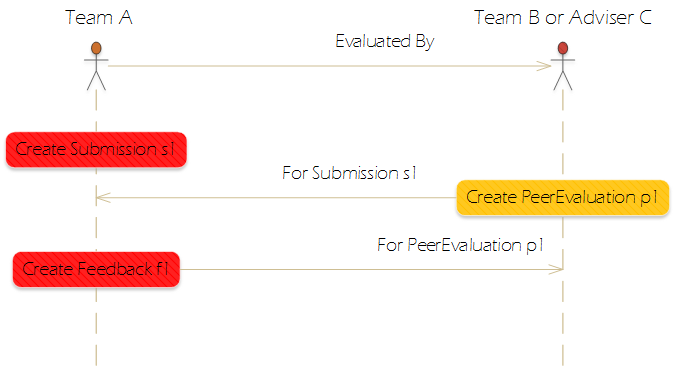
\includegraphics[width=0.85\textwidth]{Images/Skylab_Evaluation_Workflow.png}
  \caption{Illustration of evaluation workflow in Skylab}
  \label{fig:EvaluationWorkflow}
\end{figure}

The scale and routine nature of the project management in Orbital necessitates the development of a project management framework to automate many functins.  This defines the scope of Skylab —-- a development project built for administrators, facilitators, advisers, mentors and students and potential students in Orbital program. It also provides students with a real-life Software Engineering training ground to learn and sharpen programming and system design skills.

\section{Challenges}

\subsection{Tight deadlines}

As the implementation of Skylab was started only at March 2015 and students started using the system at May 2015, there was not much time for the core development. In fact, many features could only be delivered and put into production right before students in the 2015 cohort used them. Chasing deadlines and fixing urgent issues during implementation, especially in the summer when students were actively using Skylab, not only brought a lot of pressure to me but also led to difficulties in system design. I made some design decisions to compromise on certain deadlines, allowing me to postpone potential problems for later implementation.

\subsection{System design}

Skylab is built using Ruby on Rails, a mature convention-over-configuration web framework. So the first challenge is to get familiar with the conventions and recommended ways of doing things in Rails community. Then Skylab can be designed into a web application on the top of the mainstream philosophy outlined by the Rails community. Another issue with the design of Skylab is that this is the first time for me to design such an application from ground up, without any guidance from any experienced Ruby on Rails developers. Therefore, it is all about trial-and-error and explore my own way. Reading books and browsing online tutorials helped a lot and luckily there are plenty of resources about Ruby on Rails development, due to its popularity.

\subsection{Evolving requirements}

Although the scope of the project is very clear and well-defined, changes in requirements are expected and did happen frequently due to the evolving features within the Skylab project and Skylab users' feedback. The challenge is to cope with all changes and sometimes adjustments to the design of system have to be made to accommodate for extensions and new requirements. Therefore agility in development and adaptability of the system is essential.

\subsection{Data migration}

Sometimes a schema migration is required as a result of change in requirements. Therefore, dealing with old data and migration of data without affecting the use of application is another challenge during the development of Skylab. Extreme attention when migrating is required as data may not be clean enough and careless migration may even cause the system to be unusable for some users.

\subsection{Security}

Security is definitely a very important perspective in web development. Although the Rails framework already handles security well by taking measures against SQL injection, XSS attacks and CSRF attacks, there are still certain vulnerabilities when not implemented well. During development of Skylab, various techniques and practices are adopted to make Skylab more secure and trustable. For example, we implemented user roles within Skylab, allowing a role based access control system to permit users to permit fine-grained control to allowed actions.

\subsection{Coding quality/maintainability}

Although currently there is only one developer constantly contributing to Skylab repository, a good development cycle which is agile enough is not only important to keep track of history and manage different issues but also convenient for developers who may join later to jump in and get started in a short time. Testing is also a very important factor when it comes to long-term maintenance. A continuous integration would also help in catching regression errors in development early and easily. Besides all mentioned above, refactoring is helpful to the maintainability and growth of Skylab.

\section{Importance of the work}

As Orbital's evaluation of students' performance is largely based on evaluations from peers, it is very important to make the evaluation process among students to be smooth and user-friendly. Before Skylab is implemented, students were supposed to copy an HTML template and modify accordingly for their project's README and log —-- then post the submission in a forum visible to other teams. For peer evaluation, they need to repeat the whole process —-- only that this time the form is a lot more complicated and harder to copy and paste. Advisers on the other hand, have to manually remove critical sections from peer evaluations by all of his/her teams before make it visible to evaluated teams. And the worst part is that admin of Orbital program needs to do these manual work as well —-- only this time the admin has to do for all the teams (more than 100) in Orbital. Even with clear instructions, many submissions and peer evaluations were still submitted in incorrect formatting.  Advisers and administrative users needed to manually fix those. Lack of standardization also leads to trouble when trying to compile a consolidated result from submissions and peer evaluations. A lot of time is wasted in the whole process and careless mistakes in copying, modifying and pasting are just inevitable. 

So Skylab is designed and implemented to make life of students, advisers and admins of Orbital program a lot easier with standardization and automation of many procedures in Orbital program. So students can just save a lot of time and effort now by simply filling and submitting required forms, instead of copying an HTML form, modifying, pasting and finally posting as a post in a forum; advisers do not have to manually take out critical sections from peer evaluation and republish posts as the whole process is taken care by the the system; admins can easily overlook and get statistics of evaluation results through admin portal as well.

\section{Objectives}

In this project, I needed to:
\begin{itemize}
  \item Enable users to login via NUS OpenID if they have NUS Net IDs already.
  \item Enable users to login via combination of email and password for those who do not have NUS Net IDs and also serve as a backup solution to NUS OpenID login.
  \item Enable ``Forget password'' feature for those who forget their password to reset their passwords.
  \item Enable users to register for Orbital program as a team.
  \item Enable users to register for Orbital program as an individual and recommend potential good partners based on their interested topics.
  \item Enable students to edit their own team's details including ``Team Name'' and ``Project Level''.
  \item Enable students to submit for Milestones or edit their previous submissions. Besides, students in the same team should be able to see changes made by teammates(For example, Team A is supped to be evaluated by Team B, Team C and Team D. Then Team B, Team C and Team D are evaluator teams to Team A and Team A is the evaluated Team to all 3 teams).
  \item Enable assignment of evaluation relationship among teams. Each team will be assigned 3 teams as evaluators.
  \item Enable students to view submissions from teams that they should evaluate(For example, Team A is supposed to evaluate Team B and Team C; Then students in Team A should be able to view submissions from Team B and Team C).
  \item Enable students to evaluate submissions from teams that they are evaluating.
  \item Enable students to view peer evaluations from peer teams and their adviser(For example, Team B is supposed to be evaluated by Team A and Team C; Then students in Team B should be able to view peer evaluations submitted by Team A and Team C for Team B). For public part of a peer evaluation, students can see response with name of the team that submitted that evaluation; As for private part, students can only see a compilation of all private-part responses without team names.
  \item Enable students to submit feedback regarding the evaluations received(For example, Team B is supposed to be evaluated by Team A and Team C; Then students in Team B should be able to submit feedback to Team A and Team C regarding peer evaluations received from each team).
  \item Enable advisers to view a list of all teams under his/her supervision and edit any of these team's details including ``Team name'', ``Project Level'' and ``Has Dropped''.
  \item Enable advisers to submit evaluations to submissions from teams he/she supervises.
  \item Enable advisers to view feedback from his/her teams.
  \item Enable advisers to view a list of all teams and students in the current cohort.
  \item Enable advisers to view, edit and delete evaluation relationships among teams he/she supervises.
  \item Enable administrators to view, edit and delete any users, students, advisers, mentors, administrators, milestones and evaluation relationships.
  \item Enable administrators to login as any user into the system to debug and oversee things.
  \item Enable listing of all staff of Orbital program and display of their public profiles.
  \item Enable listing of all teams that passed Orbital program and display of the team's basic information.
  \item Add notion of cohort to Orbital program so that Skylab can serve for Orbital program for different cohorts.
  \item Enable admins, mentors and admins to batch send reminder emails to students and keep a history of past emails sent for checking.
\end{itemize}

\section{Outline}

In this report, I will discuss various accomplishments I have done in the development of Skylab. Chapter~\ref{background} will be an overview of current architecture of Skylab, and methodologies I employed during the development. Chapter~\ref{workflow} will be talking about solutions to problems in the implementation of registration and evaluation process. Admin portal will be discussed in details in Chapter~\ref{adminportal}. Chapter~\ref{publicprofile} will be focused on implementation of public profiles of staff and projects in Skylab. Then security related issues such as user authentication and access control will be discussed in Chapter~\ref{security}. Chapter~\ref{testing} is about how testing is done during the development of Skylab to ensure correct behaviors of various functionality and also feedback received from the focus group meeting with advisers in Orbital program. Last but not least, a summary of work and an overview of future development ends the report in Chapter~\ref{conclusionandfuturework}.
 % Introduction

\chapter{Background} \label{background}

Skylab is built using Ruby on Rails, a well-known web development framework with a great support from a large community, used widely in the industries by companies like Twitter, Groupon, Bloomberg, Airbnb and many more\cite{citation1}. There are many reasons why we have chosen Ruby on Rails. Firstly, Ruby is clean, elegant and easy to read and readability and elegance of Ruby enables programmers to be more productive. Secondly, Ruby on Rails is adopting many advanced industrial conventions and this enables contributors to have good exposure to programming in the industry. What is more, scaffolding and many gems in Ruby community can significantly simplify programmers` work by saving time and effort in ``reinventing the wheels''. And the popularity and activeness in Ruby on Rails` community ensures that getting continuous support would be easy and many resources can also be available online. Last but not least, Ruby on Rails community has a favor for open source contribution which aligns well with the open source nature of Skylab.

For the selection of database, we used PostgreSQL. Part of the reason is that it is open source and quite mature, with good drivers available in many languages\cite{citation2}. Besides, we need full ACID(atomicity, consistency, isolation and durability) compliance for consistency of data and we do not need scalability to multiple servers in the foreseeable future\cite{citationACID}. And PostgreSQL has recently added implementation for rich data structures such as JSON which would make development much easier\cite{citation3}.

Puma is the web server we have chosen for Skylab. Among common Ruby web servers such as Passenger, Unicorn, Rainbows! and Puma, Puma is considered to be fast and memory friendly according to online benchmarking\cite{citation4}. Puma is built for high-concurrency and speed and more and more developers to switching to Puma in Rails community\cite{citation5}.

We have selected Nginx as our HTTP server. Nginx has grown in popularity since its release due to its light-weight resource utilization and its ability to scale easily with low memory usage. It excels at serving static content quickly and is designed to pass dynamic requests off to other software that is better suited for those purposes\cite{citation6}. There are also some benchmarking results that indicate the superiority in Nginx handling concurrent access and low memory usage of Nginx\cite{citation7}.

A high-level overview of the architecture of Skylab is illustrated in Figure~\ref{fig:Skylabarch}. Incoming requests to server will first be forwarded to Puma worker processes by Nginx. After that the corresponding Skylab code in Ruby on Rails framework will be executed and when accessing database is required, PostgreSQL will come into picture and serve the data.

\begin{figure}[h]
  \centering
  \includegraphics[width=0.85\textwidth]{Images/Skylab_Arch.png}
  \caption{Architecture of Skylab}
  \label{fig:Skylabarch}
\end{figure}

\section{System design}

\subsection{MVC pattern in Ruby on Rails}

The basic MVC structure of Rails is shown in Figure~\ref{fig:RailsMVC}:

\begin{figure}[h]
  \centering
  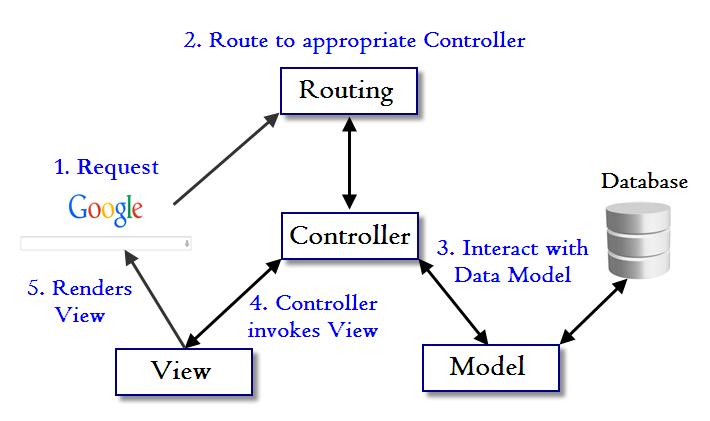
\includegraphics[width=0.85\textwidth]{Images/Rails_MVC.png}
  \caption{Illustration of how MCV works in Rails. Excerpted from \cite{citationMVC}}
  \label{fig:RailsMVC}
\end{figure}

After request is received by Ruby on Rails framework, the router will look at the pattern of the requested URL path and send it to the corresponding method of the target controller class. The controller is supposed to query models and gather necessary information for rendering the view. Last but not least, the response will be sent back to user for viewing.

So the most fundamental component in this whole process is model, which stores all the business data. A good design of model can in fact save a lot of trouble when it comes to writing controllers.

\subsection{Overview of Models in Skylab}

An overview of current models` design would be as Figure~\ref{fig:SkylabER}(source available at \cite{citationERSource}).

\begin{figure}[h]
  \centering
  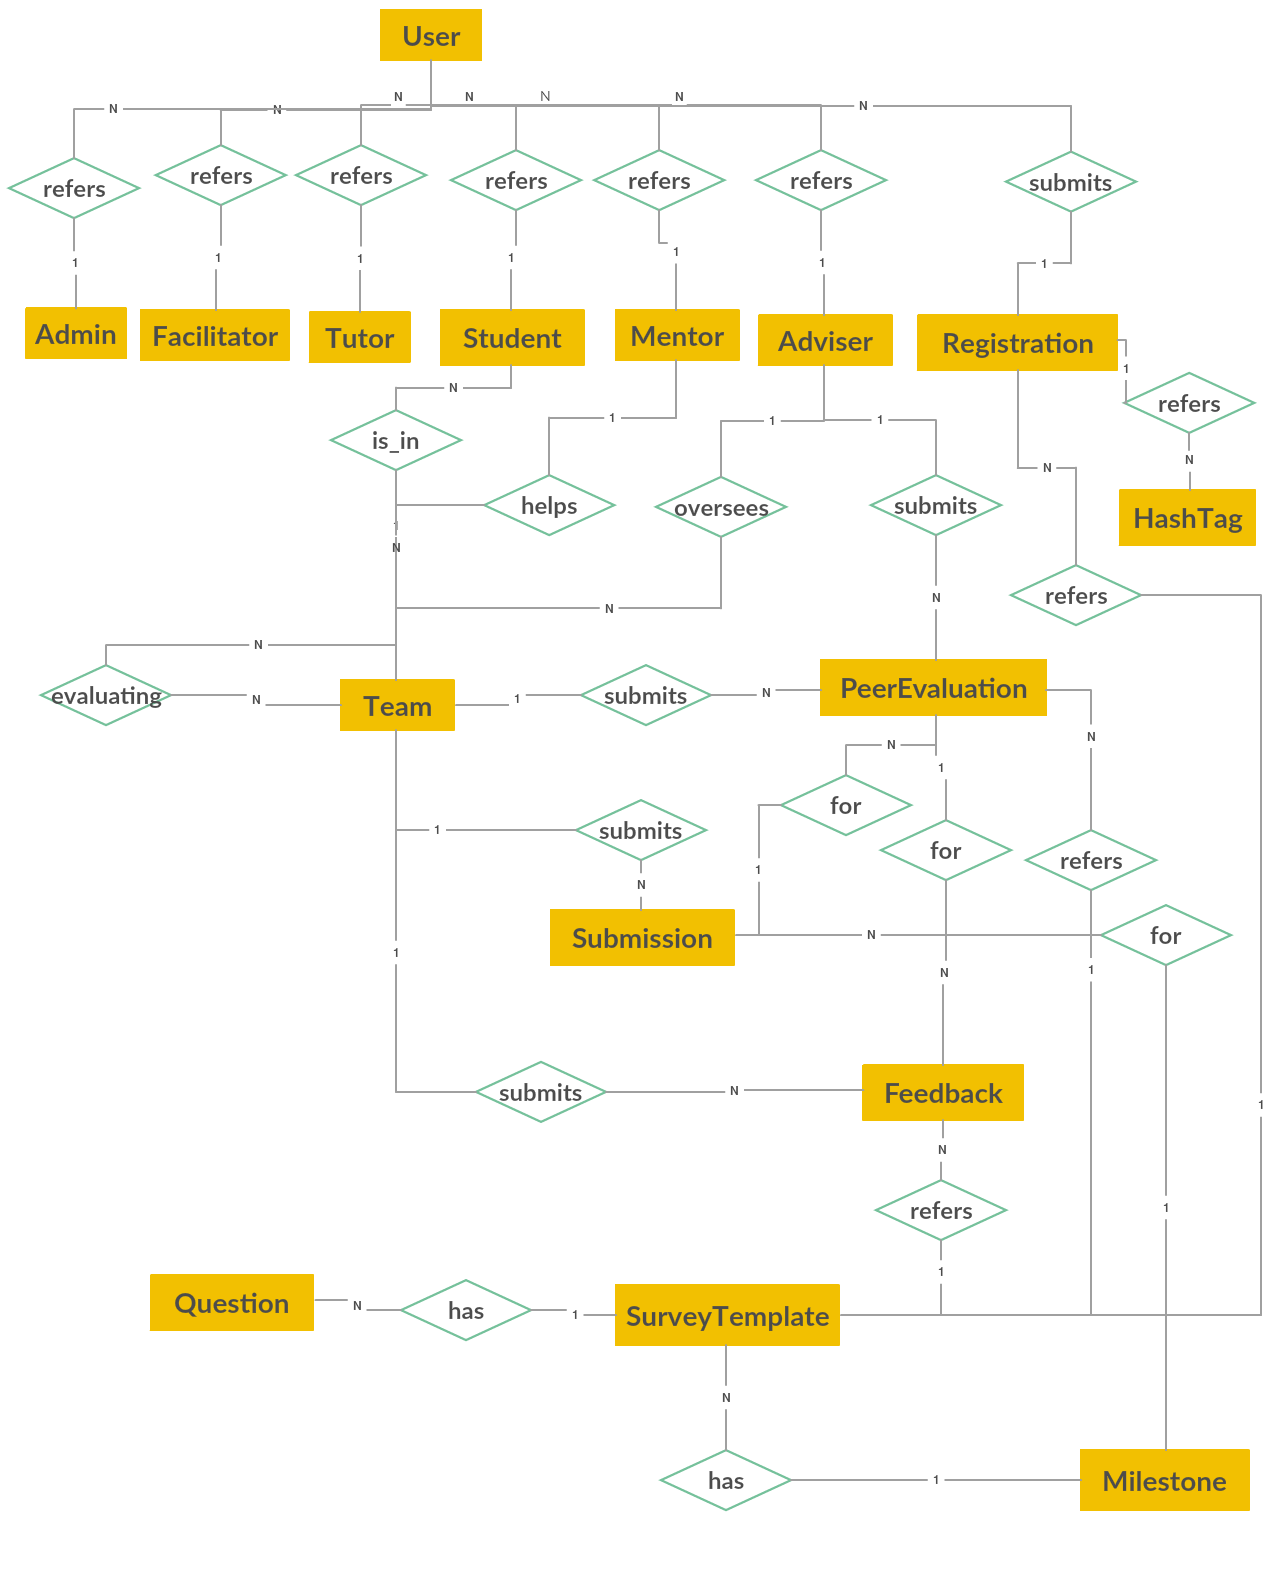
\includegraphics[width=\textwidth]{Images/Skylab_ER.png}
  \caption{Current ER diagram for Skylab}
  \label{fig:SkylabER}
\end{figure}

As you can see from the entity relation diagram shown in Figure~\ref{fig:SkylabER}, users' basic information is captured in the \textit{User} model and each user may have different roles such as \textit{Admin}, \textit{Student}, \textit{Adviser}, \textit{Mentor}, \textit{Tutor} and \textit{Facilitator}. Each user can have only one of any role in a cohort —-- meaning that if \textit{User} A is an \textit{Adviser} B for cohort 2015, then he/she's adviser role for cohort 2015 will only be B. But for cohort 2016 if \textit{User} A is an adviser again, then it is another \textit{Adviser} role C. Roles like \textit{Facilitator}, \textit{Tutor} do not have practical meanings in the system but only for display in public staff page. \textit{Admin} is supposed to overlook manage everything in Skylab. The remaining roles, \textit{Adviser}, \textit{Mentors} and \textit{Student} are connected via different relationships.

Each student has a \textit{Team} and a team has an \textit{Adviser} and a \textit{Mentor}(optional, only if the team requested). A group of teams under the same adviser is called an \textit{Evaluation Group} and evaluating relationships will be assigned from team to team in the same \textit{Evaluation Group}. Each team will create \textit{Submissions} to \textit{Milestones} to report their progress and their adviser and assigned evaluator teams will submit \textit{PeerEvaluations} to the team`s \textit{Submissions}. A \textit{SurveyTemplate} contains \textit{Questions} for a \textit{Feedback}, which is for evaluated team to provide feedback to their evaluator teams. After receiving the \textit{PeerEvaluation}, the team is supposed to submit \textit{Feedback} to rate the helpness of received \textit{PeerEvaluations}.

Before Orbital officially starts, interested students need to register in Skylab first. A \textit{Registration} will be created to record information about the student and his/her interested topics of project in the summer for recommending potential teammates if they do not have a partner in mind at the time of registration. \textit{Registration}, \textit{PeerEvaluation} and \textit{Feedback} will all make references to a \textit{SurveyTemplate}, which contains some \textit{Questions} to be answered.

\subsection{Overview of Controllers in Skylab}

Controllers will query models to get information needed to present views or make modifications to models if requested. Therefore they are crucial in powering a Rails application and in Skylab we have well-defined controllers to carry out different tasks. A class digram of all controllers in Skylab is shown in Figure~\ref{fig:SkylabControllers}.

\begin{figure}[h]
  \centering
  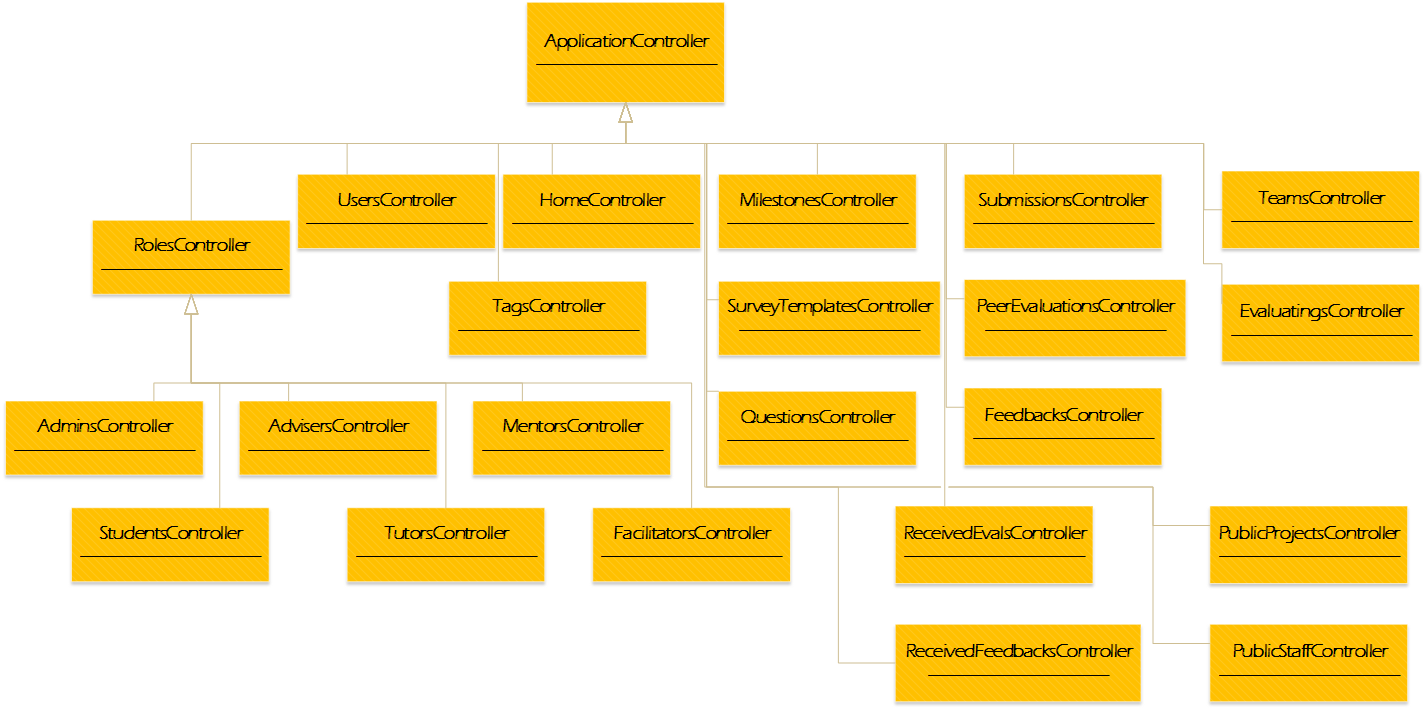
\includegraphics[width=\textwidth]{Images/Skylab_Controllers.png}
  \caption{Current Class diagram of controllers in Skylab}
  \label{fig:SkylabControllers}
\end{figure}

ApplicationController is the base of all other controllers. Utility methods such as access control, page title and handling of exceptions are included in ApplicationController and it also includes auxiliary modules such as CohortHelper to enrich its functionality. RolesController is the base class of all roles` controller classes: AdminsController, AdvisersController, MentorsController, StudentsController, FacilitatorsController and TutorsController. These roles share quite a lot in common so they will share request processing methods and they will override data related methods or provide some handlers for special cases. Other controllers are as follows:

\begin{itemize}
  \item \textbf{HomeController}: serves home page to user only.
  \item \textbf{UsersConroller}: manages listing, creation, editing and display of users and also includes functionality for admin to masquerade as any user, for new users to register as students in Orbital.
  \item \textbf{TagsConroller}: lists tags based on specified filters.
  \item \textbf{MilestonesConroller}: handles listing, creation, editing and display of milestones.
  \item \textbf{SurveyTemplatesConroller}: handles listing, creation, editing and display of survey templates and also serves as interface for editing of questions belonging to current survey templates. 
  \item \textbf{QuestionsConroller}: manages Ajax requests to create, edit or delete a question.
  \item \textbf{SubmissionsConroller}: manages creation, editing and display of submissions by students.
  \item \textbf{PeerEvaluationsConroller}: handles creation, editing and display of peer evaluations from evaluator teams or advisers to evaluated teams.
  \item \textbf{FeedbacksConroller}: manages creation, editing and display of feedback from evaluated team to evaluator teams or advisers.
  \item \textbf{ReceivedEvalsConroller}: compiles a set of received peer evaluations for a team in one milestone.
  \item \textbf{ReceivedFeedbacksConroller}: compiles a set of received feedback for a team or an adviser in one milestone.
  \item \textbf{PublicProjectsConroller}: serves completed teams` projects to the public.
  \item \textbf{PublicStaffConroller}: serves staff of Orbital program to the public.
  \item \textbf{TeamsConroller}: manages listing, creation, editing and display of teams.
  \item \textbf{EvaluatingsConroller}: handles listing, creation, editing and display of evaluating relation among teams.
\end{itemize}

Controller manages a collection of \textit{resources} in Skylab, meaning that each controller is managing(list, create, edit and display) usually one model class only for higher cohesion. If dependency on other models is needed, for example, SurveyTemplate will manage questions belonging to current SurveyTemplate, the requests will be handled by Ajax requests to separate concerns.

Skylab is following Ruby on Rails convention for controller classes. A basic controller that manages a collection would have the following structure illustrated in Figure~\ref{fig:SkylabSampleController}.

\begin{figure}[h]
  \centering
  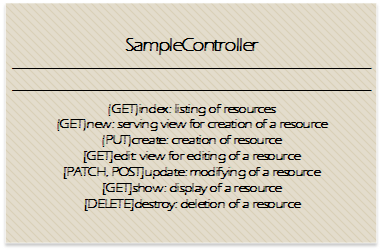
\includegraphics[width=0.6\textwidth]{Images/Skylab_Sample_Controller.png}
  \caption{Sample controller class in Skylab}
  \label{fig:SkylabSampleController}
\end{figure}

These methods —-- index, new, create, edit, update, show and destroy —-- have included all the basic actions to be done with a collection of resources. Following such a convention would not only make controller class in Skylab consistent and easy to read, but also align well with a more human-readable RESTful URL design.

\section{Development process}

As Skylab is a web application for which version does not mean anything in particular, we have adopted GitHub flow in our development process\cite{citation8}. So the master branch always contains the latest stable and deployable code base. Each feature will be developed on a feature branch and once the feature is ready, a pull request is created against master. After code review and all tests passes, pull requests will be merged into master and ready for deployment. Figure~\ref{fig:GithubFlow} illustrates the process as well.

\begin{figure}[h]
  \centering
  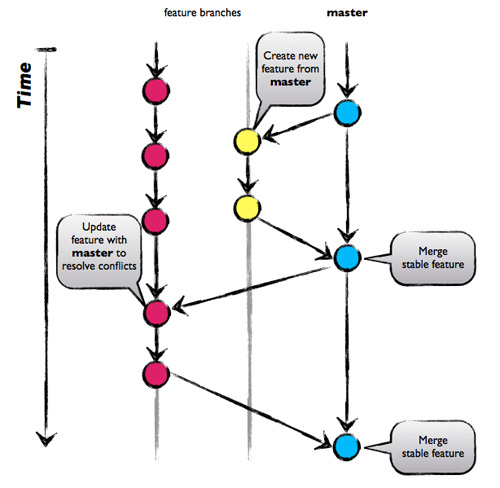
\includegraphics[width=0.85\textwidth]{Images/Github_Flow_Branching_Model.png}
  \caption{Branching diagram for GitHub Flow. Excerpted from \cite{citation8}}
  \label{fig:GithubFlow}
\end{figure}

By using GitHub flow and services such as Travis as the continuous integration service, CodeClimate as the code quality monitoring service, we can keep the development of Skylab agile and fast. Besides GitHub flow has enabled Skylab to deployed regularly, which is essential for timely improvement of user experience\cite{citation9}.
 % Background

\chapter{Orbital workflow} \label{workflow}

To appreciate the scope of the design and implementation Skylab, we detail the major work processes that the various user roles need to accomplish during an iteration (one year's cohort) of Orbital.  We describe the workflow for Orbital students first, and circle back to describe the workflows of other supporting roles in the process.

\section{Registration} \label{registration}

To enroll in the Orbital program, students will need to register in Skylab first. When a user first logs into Skylab, a \textit{User} object will be created for user. And since it is the first time the user logs in to the system, there is no existing role assigned to current user in current cohort. Then Skylab assumes that the user is trying to register and therefore a link to registration will be displayed. This workflow works for most users who are students in Orbital program. As for roles like \textit{Adviser}, \textit{Mentor} and \textit{Tutor}, admin users will create those roles manually. This is because there are only a few such roles and they have higher privileges and therefore creation of such roles should definitely be controlled by admin users.

For students' registration, after a user click the registration link, a form consisting of different questions will be presented to the user. Among these questions, several are to get a sense of what sort of interests the user has for the project over the summer. The user is supposed to select interested topics from different categories like programming language, web framework or mobile platform, IDE or text editor, e-commerce, cloud platform, purpose, embedded system, game framework, content management system and audience. These information will be recorded for match-making among students who need to find a teammate in Skylab.

After completing the registration form, if the user already has a teammate in mind, he/she can send an invitation to the potential teammate to form a team. Some users, on the other hand, do not have anyone to partner with for Orbital yet and a match-making algorithm will be run offline by admin user based on the interested topics they have selected during registration. An illustration of the whole workflow is as Figure~\ref{fig:RegistrationWorkflow}.

\begin{figure}[h]
  \centering
  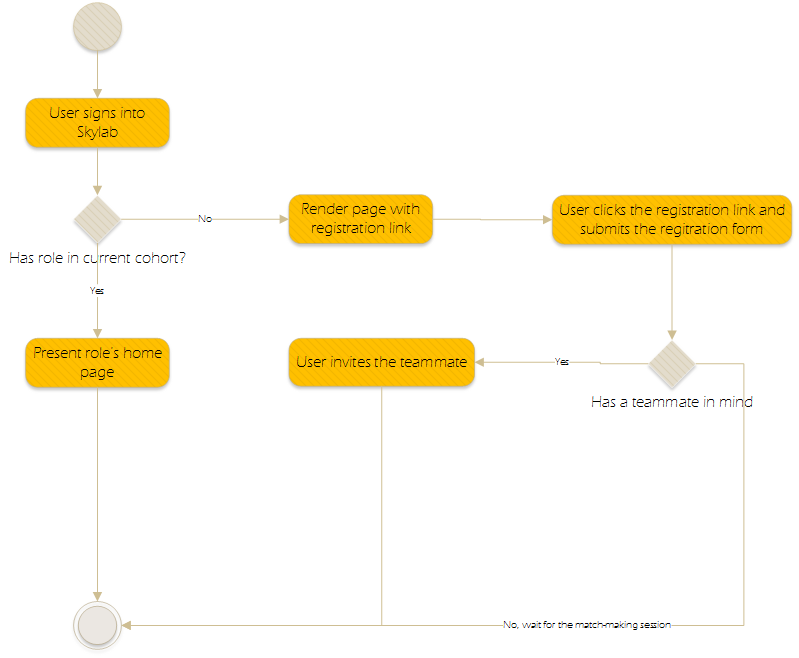
\includegraphics[width=\textwidth]{Images/Skylab_Registration_Workflow.png}
  \caption{Illustration of registration workflow in Skylab}
  \label{fig:RegistrationWorkflow}
\end{figure}

\subsection{Match making algorithm}

For students who do not have potential teammates at the time of registration, we will run a matching making algorithm based on the interested topics recorded in registration form submission. The algorithm composes of mainly two steps:

\begin{itemize}
  \item Calculate inverse document frequency of tags: inverse document frequency is to reflect how rare a term is in the corpus\cite{citationir}. In Skylab's match making's case, a document is a user's selection of interested topics, or tags; the corpus is the collection of users' interested topic sets; a term is a tag in a users' selections. If a term(tag) is rare among registration form results, we will be more confident that if both students choose this term and they will have higher chance of forming a team. The formula of calculation is as Formula~\ref{eq:idf}.

  \begin{equation}
    idf(t,D) = \log \frac{N}{\{ d \in D : t \in d \} + 1} \
    \label{eq:idf}
  \end{equation}
  
  with \(N\) as total number of documents in the corpus \( N = |D| \) and \(\{ d \in D : t \in d \}\) as number of documents where the term \(t\) appears\cite{citationir}.

  \item Construct a vector space model based on students' selected tags and each tag's weight calculated in previous step and calculate similarity(cosine) of different students. The formula for calculating cosine of two vectors is as Formula~\ref{eq:veccos}\cite{citationvecspacemodel}.

  \begin{equation}
    \cos\theta  = \frac{d_2 \cdot q}{ \norm{d_2} \norm{q} } \
    \label{eq:veccos}
  \end{equation}

  And we represent a user's interested topics with tags' weights and the similarity between 2 users will be the cosine between 2 vectors representing the 2 users. The formula for calculating cosine of two vectors is as Formula~\ref{eq:similarity}\cite{citationvecspacemodel}.

  \begin{equation}
    sim(d_j, q)  = \frac{d_j \cdot q}{ \norm{d_j} \norm{q} } \ = \frac{sum_{i=1}^{N} \omega_{i,j} \omega_{i,q}}{ \sqrt{sum_{i=1}^{N} \omega_{i,j}^2} \sqrt{sum_{i=1}^{N} \omega_{i,q}^2}} \
    \label{eq:similarity}
  \end{equation}

\end{itemize}

As matching making only needs to be run once before Orbital officially starts for those students who do no have a team yet, the algorithm is currently designed to run offline as a rake task. Currently it is only for students but in the future with recoding of mentors' and advisers' interested tags, this algorithm can be easily extended to students and mentors or students and advisers as well.

\section{Submission} \label{submission}

Students in Orbital are supposed to report their progress regarding their project at each milestone via \textit{Submission}. Basically a submission contains 3 parts:

\begin{itemize}
  \item README: highlights what are the changes and new features in the project.
  \item Project Log: a summary of work done during the phase and time used for each task.
  \item Video link: a link to a video introducing the project to evaluators.
\end{itemize}

As the structure of \textit{README} and \textit{Project Log} is free and we should allow creativity of students when it comes to describing their own projects, we decided to support rich text for submissions and there are some issues coming along with this decision such as SQL injection and XSS attacks. What is more, during use of Skylab, many good suggestions regarding user experience were brought up by students and advisers, like uploading of images and auto-expanding textareas during editing.

\subsection{Handling of rich text}

We used TinyMCE to support rich text editing feature in Skylab as it is a very popular WYSIWYG(what-you-see-is-what-you-get) editor with a rich set of features\cite{citationtinymce}. There are some libraries with markdown syntax supported such as EpicEditor, Vue.js and Hallo.js which are more lightweight. However, as Skylab is built for freshmen to get more hands-on experience with coding, we do not expect students to be equipped with much prior knowledge such as markdown syntax. In the contrast, markup based editors such as TinyMCE and CKEditor do not require any learning and are easily to get started with. What is more, the large community using TinyMCE has made various plug-ins available for different features. There are also quite good resources online about integrating TinyMCE editor in a Rails project. Therefore, we decided to use TinyMCE for \textit{Submissions}' rich text support.

One particular disadvantage of using TinyMCE is that the size of this editor is pretty large and loading of the page will be slowed down because of it. Therefore, TinyMCE related resources is only loaded if the page is requiring rich text editing. This is done by configuration to disable auto loading of all JavaScript, which is the default behavior of Rails. In this way, most pages can be loaded within a very short time. What is more, assets whose names start with ``tinymce'' are set to expire in a year to reduce frequent requesting of such resources from clients --- which basically means students only need to load these resources once in one year.

Rails has built-in checking against SQL injection attacks and therefore Skylab is safe from such attacks when storing submissions' contents\cite{citationrorsecurity}. However, there is still currently a known bug in the implementation when it comes to viewing of submissions. As contents like \textit{README} and \textit{Project Log} should be rendered as rich text, it is possible for students to perform XSS attacks by injecting executable JavaScript code in the submission. This sort of vulnerabilities will be fixed in the future.

\subsection{Usability}

Skylab is a software engineering project and therefore improvements in user experience is one key part when it comes to implementation. During the use of Skylab, many suggestions were brought up by students and advisers about usability. And by addressing these issues, Skylab is serving users better with a smoother user experience.

\subsubsection{Target Milestone Selection}

When Skylab was used for the first time, students were expected to choose the target milestone, which the submission is for. However, many students reported that it is just a redundant step as every time they will only submit to the currently active milestone. After hearing this, a quick fix of automatically selecting the current milestone for students using JavaScript functions was done, while the manual selection is still possible. And then during the \textit{Adviser Focus Group Meeting}, some advisers further pointed out that the selection should not even be presented to users as it is of completely no use and therefore the whole selection was completely removed from Skylab after the meeting by moving the task to the backend logic. 

\subsubsection{Rich Text Editing}

As quite some students want to insert image to \textit{README} sections, an image uploading feature was soon added to submission page for users' convenience. Behind the scene Skylab is using a third-party API from Imgur. This was done mainly for 2 reasons: using Imgur is relatively easy to implement; we can also avoid heavy server load due to file uploading and possible attacks in uploaded files.

Another improvement over user experience is auto expanding of TinyMCE editing area as feedback from students mentioned that their \textit{README} and \textit{Project Log} are usually quite lengthy. So auto expanding would not require too much scrolling during creating/editing a submission.

\section{Peer Evaluation} \label{peerevaluation}
 
 After students have submitted to milestones, peer evaluation process can begin. Teams will look through evaluated teams' projects and submissions and then evaluate their performance in \textit{PeerEvaluation}, which is a very important component in determining whether the evaluated teams can pass Orbital or not. Although there are different questions for each peer evaluation, all evaluations contains essentially 2 parts:

 \begin{itemize}
  \item Public: a section with general feedback on how well the evaluated team has done and the response will be viewed by target team with evaluator team name available.
  \item Private: a section with critiques and overall rating. Critiques will only be viewed by target team without any evaluator team information while overall rating is only for grading purpose and not viewable by target teams.
\end{itemize}

\subsection{Loading of Peer Evaluation templates}

When Skylab was first developed, the public part of a \textit{PeerEvaluation} templates will be one HTML form and the private part is another one. This means all questions in the public part are coded in one predefined html template and same goes for questions in private part.

This approach does not seem to have much problem at first and it really served Skylab's purpose well by delivering perfectly workable features in time. However, since questions are different for different milestones, separate templates have to be created for each new milestone. And when user wants to view/submit/edit a \textit{PeerEvaluation}, the corresponding templates will have to be loaded based on properties of the milestone. In this way, the system is not really open to extension and clearly it violates Open-Close principle. After realizing this, a system for dynamically creating questions has been implemented for \textit{Feedback} and migration of \textit{PeerEvaluations} to the survey-template-and-questions based system has been done as well. A more detailed description for how the dynamic loading of questions is in Section~\ref{feedback}.

\section{Feedback} \label{feedback}

\textit{Feedback} is for evaluated teams to evaluate the \textit{PeerEvaluations} they have received and it is also a very important component in determining whether the evaluator team can pass or not. After realizing the lack of extensibility in the design for \textit{PeerEvaluations} and with more time available for implementation of \textit{Feedback}, a survey-template-and-questions system has been set up, which made the system open to extensions for more questions and even question types.

\subsection{Survey-template-and-questions system}

The basic flow when a request to create a \textit{Feedback} is illustrated in Figure~\ref{fig:FeedbackFlow}.

\begin{figure}[h]
  \centering
  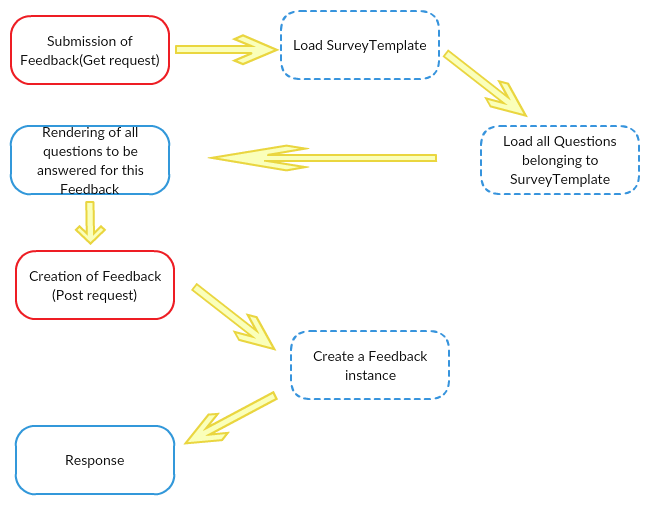
\includegraphics[width=0.8\textwidth]{Images/Skylab_Feedback_Flow.png}
  \caption{Flow of a feedback creation process}
  \label{fig:FeedbackFlow}
\end{figure}

So when a student clicks the button to create feedback, \textit{FeedbacksController}'s \textit{new} action will be invoked and inside the method, the corresponding \textit{SurveyTemplate} and all \textit{Questions} belonging to the \textit{SurveyTemplate} will be sent to view. Then instruction for the \textit{Feedback} and all questions will be rendered as response to the student. After the student completed and pressed submit button, responses to all questions will be sent to server and a Feedback instance containing all submitted responses will be created.

There currently 4 types of \textit{Questions} in the system as Figure~\ref{fig:SkylabQuestions}:

\begin{itemize}
  \item \textbf{TextQuestion}: a text question which will be rendered in the format of textarea and text-based responses are expected. 
  \item \textbf{RichTextQuestion}: a rich text question which will be rendered in the format of TinyMCE editable area and rich text is expected as response.
  \item \textbf{MultipleChoiceQuestion}: a multiple choice question which will be rendered as radio buttons followed by option descriptions and one option value is expected.
  \item \textbf{MultipleSelectQuestion}: a multiple choice question which will be rendered as a select element with ``multiple'' enabled with each option as one choice of selection.
\end{itemize}

\begin{figure}[h]
    \centering
    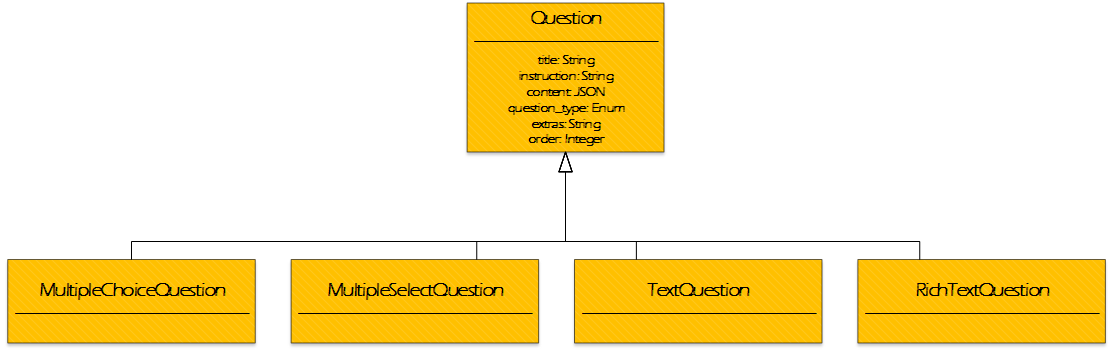
\includegraphics[width=\textwidth]{Images/Skylab_Questions.png}
    \caption{All types of questions in Skylab}
    \label{fig:SkylabQuestions}
\end{figure}

All types of question will have \textit{title}, \textit{instruction}, \textit{content}, \textit{extras} and \textit{question\_type} and each type of question will have its own way of rendering and validation. In this way, adding new types of questions can simply be done via creating a new question model with its own rendering and validation methods.
 % Orbital workflow

\chapter{Admin Portal} \label{adminportal}

Admin users are supposed to overlook everything in Skylab to monitor progress of students and performance of different teams and advisers. Therefore they have the highest privileges in Skylab. And due to the fact that admin users have so much to do in Skylab, a lot of effort has been put into the development and improvement of functionalities related to administration.

\section{Overview and export} \label{adminoverview}

To oversee and manage different perspectives of Skylab well, admin users need to have access to all information in Skylab in a easy way. In Skylab, the basic steps for an admin user to have an overview of something is simply to navigate through navigation header and after that a table consisting of brief information about each record in the collection will be presented in a table`s form. For example, if the admin user wants to view all the students in current cohort, he can simply press the link in the navigation header and students in the current cohort will be listed with basic information such as name, email, team, adviser, is\_pending. Also for each student, the admin user can get more information by clicking view to go to the student`s page or edit the student`s some information.

Sorting of records in the table is provided for admin users to quickly rank students via some condition. However, filter is not implemented as of now as admin users are considered to be skillful and familiar with the data and mainly use ``Find'' functionality provided by the browser to locate some record.

To enable admin users to do more things with the data, exporting feature has been implemented for students and teams as well. After getting data exported as CSV, admin users can use text editors or Excel to manipulate the data further. Although ideally some features could be added to Skylab so that admin users can just do it in the system without extra steps, due to the time limit and other tasks, exporting data is a quick way to get admin users to carry out desired tasks.

\section{Preview as other users} \label{adminpreviewas}

Admin users can view any user`s information for overlooking. And there is not more functionality for admin to ``fake login as'' any other user. During development of Skylab, checking student`s view and adviser`s view is needed by the developers a lot to see whether user interface is in the desired way. What is more, admin users can also use this feature to actually go through flows of user`s action needs adjustment or not and through the implementation of Skylab, many good suggestions about user experience enhancement have been by admin users thanks to this. Besides these, ``fake login as'' can help admin see the issues reported by students and advisers in production environment so that the fixing can be faster and more targeted.  

\section{Mailing} \label{adminmailing}

Mailing is a very important feature for admin users as many reminders and announcements should be delivered to users` emails for them to check. So there are basically 2 types of emails sent in Skylab.

\begin{itemize}
  \item Reminder emails: this sort of emails do not require admin users` actions to be sent to users, for example, forget-password emails to reset password, welcome email when admin users create a user, reminder emails when deadlines are coming for submission, peer evaluation and feedback.
  \item User-initiate emails: this type of emails are written by users and sent at users specified timings and would serve as the channel for general reminders and announcements. And these emails will be recored as history so that user can look at past records to compose a similar email. This feature is not limited to admin users and in fact advisers are also allowed to use this to remind students in his/her evaluation group.
\end{itemize}

Admin users can make use of mailing to remind students and this can save admin`s time and effort in manually sending emails. It can also serve as an alternative to existing communication tools such as Slack in case some students ignored those discussions.
 % Admin portal

% Min: seems too short to be a chapter.  Fold it in some other chapter?
\chapter{Public Views} \label{publicprofile}

Before Skylab was implemented, the display of past Orbital staff and projects was done by means of a manually curated WordPress post.   Project links for teams and team members were all manually created, which was a tedious and error-prone process. Since Skylab already captures all information on teams and students, publicly-accessible (i.e., without needing to login) pages are a logical form of data export that has been created to supercede these past facilities.

\section{User Avatars} \label{useravatar}

Skylab does not currently handle image uploading, as it requires a lot more storage and more efforts in security as well. However, we need to support user avatar pictures as this enhances the user experience of Skylab.  To implement this, we have integrated with an external third party service.   We have decided to use Gravatar, a globally recognized avatars for users\cite{citationgravatar}. Gravatar is popularized by Wordpress and in use by many sites.  It is easy to integrate and a number of users already use gravatar for creating a universal user avatar for themselves.  The steps to get a gravatar are as follows:

\begin{itemize}
  \item Trim the user's email address, convert it to lower case, and calculate MD5 hash of the transformed email address.
  \item Use the hash computed in previous step and append it to \url{http://www.gravatar.com/avatar/} to obtain the gravatar's image source.
\end{itemize}

Gravatar serves our purpose of serving users' avatars while bypassing the complication of supporting image uploading and storage, as this is handled by the service. And the most important part in arriving at this solution is that it is a relatively quick, easy yet clean to serve users' profile images. Compromises like this happen as we need to weigh advantages and disadvantages of different approaches and take the time taken and priority of issues in implementation into consideration. In the future, if we find too many inconveniences from using Gravatar, we may decide to host avatar images on our own server, and handle problems arising from the support of file uploading and storage.
 % Public profile

\chapter{Security} \label{security}

During the development of Skylab, security has always a priority. Common attacks such as SQL injection, XSS attacks and CSRF attacks are all partially addressed by the Rails framework itself. Skylab's main security focus is to make sure authentication process and access control are well-defined and can withstand various attacks.

\section{User authentication}

There are basically 2 ways to login to Skylab: email and password combination and NUS OpenID. For email and password combination, we employ Devise to manage authentication related information in \textit{User} model. Devise has been used widely in Rails community and currently there are more than 13,000 stars of Devise repository on GitHub\cite{citationdevise}. What is more, according to security scanning of Devise by Hakiri there is no security warning, which further proves the trust-ability of Devise\cite{citationdevisehakiri}. As for NUS OpenID, it is using OAuth 2.0 as authentication protocol, which is believed to be safe and currently is adopted by many OpenID providers as well\cite{citationnusopenid}.

\section{Access control}

Skylab is adopting role based access control strategy to grant different permissions for different users. There are basically 4 levels of checking for each incoming requests:

\begin{itemize}
  \item \textbf{login\_required:} a boolean value. If a action is login\_required then a user must sign to be granted for the access.
  \item \textbf{admin\_only:} a boolean value. If a action is admin\_only then only users with role of \textit{Admin} can access; but if current user is admin, the next check will be skipped and return true directly as admin users can access any resources in Skylab.
  \item \textbf{allowed\_users:} a boolean value. If a action requires login and is not only accessed by admins, then the current logged-in user will be checked against the list of allowed users who have the permissions.
  \item \textbf{strategy:} a lambda function which can be executed and is expected to return a boolean value. If the lambda is provided by the caller, it will be executed and whether users in allowed\_users can actually access the resource or not depends on the returned result.
\end{itemize}

As this checking procedure is a common to nearly all actions, it is defined in \textit{ApplicationController} which will be effectively inherited by all controllers in Skylab. So all methods in those controllers can invoke this method to check user's permission first.

\section{Security warnings}

Hakiri is used as the security analysis tool in Skylab. Currently there are some warnings in cross-site scripting, code injection, file access, input validation, resource management according to Hakiri scanning result. However, all of these security issues are actually vulnerabilities in current version of Ruby on Rails framework used by Skylab --- so this means that by upgrading the Rails framework we can simply remove these issues.

\begin{figure}[h]
	\centering
	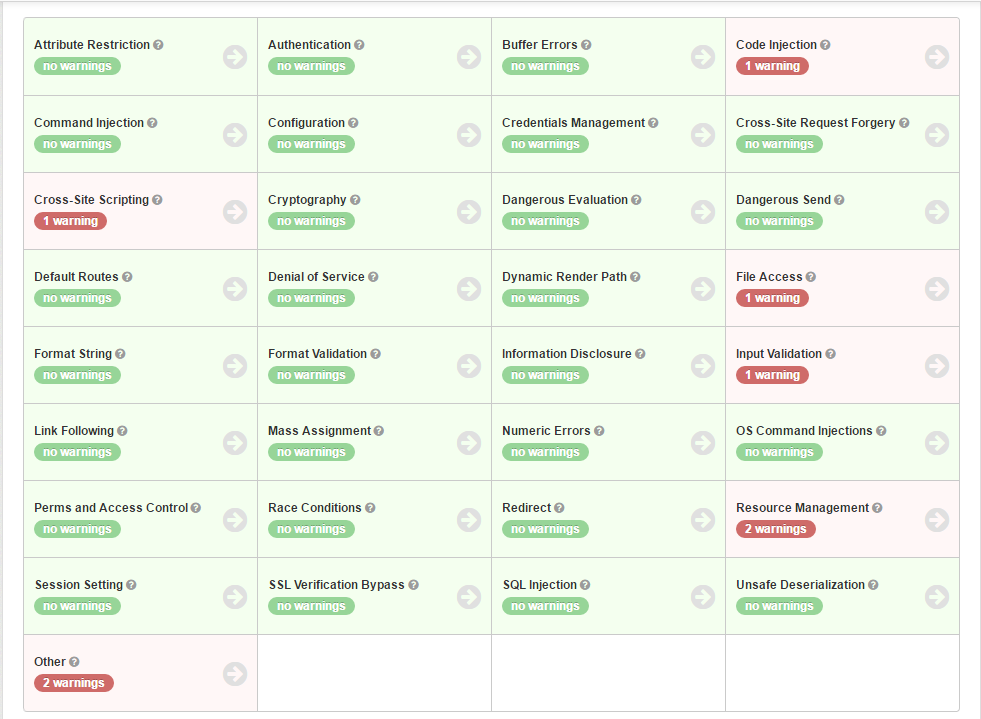
\includegraphics[width=\textwidth]{Images/Skylab_Hakiri.png}
	\caption{Hakiri security warnings}
	\label{fig:SkylabHakiri}
\end{figure}

Due the importance of security in the development of a web application, security will remain as an prioritized task in Skylab and more future work will be done regarding this as well.
 % Security

\chapter{Testing} \label{testing}

Testing is very important in development as it serves as the validation and verification of the program\cite{citationtesting}. And also in the process of continuous development, having tests can help us catching errors, especially regression errors. Skylab as a software engineering project, is covered by different level of tests to make sure the delivered features are as promised.

Testing in GitHub flow —-- the development process adopted in Skylab —-- has a special place as well. Through continuous integration tools like Travis, each pull requests and commits on master branch will be tested and the status will be used as the indicator whether merging to master brunch should be done and the health of current master brunch.

Rspec is the testing library used in Skylab and it is widely used the testing tool for many Ruby on Rails programmers as well\cite{citationrspec}. And for database testing, FactoryGirl is used for creating records in databases. The syntax of FactoryGirl and Rspec is pretty expressive and concise, which aligns well with design of Ruby on Rails and helps to improve readability of testing code.

\section{Unit testing} \label{unittesting}

Models are the most fundamental components in Ruby on Rails` MVC pattern and they are tested and covered fully in Skylab. In Skylab, models` testing are executed on testing database instead of faking models to test logic and validation in models only. Although this would slow down execution of test suite overall as database access is usually slow, we want to make the integration of models` logic and constraints in database just would work as expected. And since currently the test suite of Skylab does not take more than 2 minutes to run, we would favor better tested code over faster execution of tests.

Controllers usually do some complicated data querying and processing so tests on controllers can fully cover as well. However, so far, helpers and mailers are not tested in Skylab now due to time limit and the fact the helpers and mailers are relatively straight forward.

\section{Acceptance testing} \label{acceptancetesting}

Acceptance testing is to make the whole system would work as expected when users carry out various of activities. Most use cases are covered in acceptance tests for Skylab like registration form submission, team invitation, admin`s overview of different models in Skylab, students` submissions, peer evaluations and feedback. Although the testing coverage in Skylab is pretty high and most use cases are included in acceptance testing as well, there are more details to check in testing and other cases like advisers` evaluations, management of evaluatings and others as well. Trying to cover more perspectives in Skylab is therefore one of the main future tasks.
 % Testing

\chapter{Conclusion and future work} \label{conclusionandfuturework}

\section{Conclusion}

Skylab is supposed to serve facilitators, advisers, mentors and students and potential students well by making experience in Orbital more pleasant. Through the whole process of Orbital program, Skylab has been playing a helpful role in registration, match making after registration, submissions of project log and README, peer evaluations for evaluated teams` submissions and feedback to peer evaluations. There are also work done on admin portal for overseeing Skylab and reminding users and public views to display past projects and staff in Orbital program.

The development process of Skylab is certainly agile and iterative. Many features are developed as prototype first and after discussion adjustments are made to have a better user interaction experience. Besides, as Skylab is continuously being used, some requirements and suggestions are made by users as well. Many challenges to system design rise in the process of changing and refining. Various compromises have to be made to due to deadlines or other important issues. During implementation of Skylab, copying with changes and deadlines is the most important skill. Designing a system with enough features, with enough good features, with enough good features and extensibility to add more good features is huge challenge and Skylab is trying to be a system with many good features and open to extensions in the future.

\section{Future work}

A proposed set of major features to be completed in the future for Skylab:

\begin{itemize}
  \item Questions/template system(involving migration of current data): currently \textit{Feedback} and \textit{Peer Evaluation} is utilizing the \textit{SurveyTemplate} and \textit{Question} system but \textit{Submission} are still not. With migration to \textit{Questions} system we can further improve the system by adding more extensibility.
  \item Implementation of more mailer actions: we can explore power of emails by sending reminder emails to students when deadlines are approaching or even embed secure link for students to submit submissions, peer evaluations and feedback without login.
  \item Logging of user activities: by logging down activities carried out by different users, users can more easily figure out what has happened and get a better sense of the context of Skylab.
  \item Acceptance testing needs cover more use cases in Skylab by different users.
\end{itemize}

 % Conclusion

%% ----------------------------------------------------------------
% Now begin the Appendices, including them as separate files

\addtocontents{toc}{\vspace{2em}} % Add a gap in the Contents, for aesthetics

\appendix % Cue to tell LaTeX that the following 'chapters' are Appendices

% \chapter{Closed Issues on GitHUb}

{\tiny
\section{V0.0.0}
\begin{itemize}[noitemsep]
    \item setup the basic rails project with ability to submit simple form of evaluation \url{https://api.github.com/repos/nusskylab/nusskylab/issues/7} 
    \item fix the bug with ip port forwarding with vagrant \url{https://api.github.com/repos/nusskylab/nusskylab/issues/3} 
    \item explore the use of rbenv for managing ruby versions \url{https://api.github.com/repos/nusskylab/nusskylab/issues/2} 
    \item setup the project env with rails@4.2 and ruby@2.2 \url{https://api.github.com/repos/nusskylab/nusskylab/issues/1} 
\end{itemize}

\section{Beta-0.0.1}
\begin{itemize}[noitemsep]
    \item edit student: auto generate matric no \url{https://api.github.com/repos/nusskylab/nusskylab/issues/24} 
    \item admin can update and delete students \url{https://api.github.com/repos/nusskylab/nusskylab/issues/22} 
    \item refactor students + users  see if we can include from another directory \url{https://api.github.com/repos/nusskylab/nusskylab/issues/21} 
    \item provide a list of all users to admin \url{https://api.github.com/repos/nusskylab/nusskylab/issues/18} 
    \item admin can delete students: either by cascade delete or code  consistence has to be maintained \url{https://api.github.com/repos/nusskylab/nusskylab/issues/17} 
    \item design user model  forming of teams  linking with milestones under orbital  prepare for submissions from users  \url{https://api.github.com/repos/nusskylab/nusskylab/issues/13} 
    \item admin can add new students  with student information provided in a form \url{https://api.github.com/repos/nusskylab/nusskylab/issues/10} 
    \item setup user system  either by using devise or setup our own user-role system \url{https://api.github.com/repos/nusskylab/nusskylab/issues/9} 
    \item add omnioauth and achieve nus openid login \url{https://api.github.com/repos/nusskylab/nusskylab/issues/8} 
\end{itemize}

\section{Beta-0.0.2}
\begin{itemize}[noitemsep]
    \item student submit via team to milestone \url{https://api.github.com/repos/nusskylab/nusskylab/issues/35} 
    \item add a series of action to teams \url{https://api.github.com/repos/nusskylab/nusskylab/issues/33} 
    \item enable individual assignment of team to a student \url{https://api.github.com/repos/nusskylab/nusskylab/issues/31} 
    \item add a series of action to mentors \url{https://api.github.com/repos/nusskylab/nusskylab/issues/30} 
    \item add a series of action to advisers \url{https://api.github.com/repos/nusskylab/nusskylab/issues/29} 
    \item update student: ensure that only one team entity exists for one team name \url{https://api.github.com/repos/nusskylab/nusskylab/issues/23} 
    \item admin can view list of mentors  advisers  and create advisers and mentors \url{https://api.github.com/repos/nusskylab/nusskylab/issues/20} 
    \item admin can assign mentors and advisers to teams \url{https://api.github.com/repos/nusskylab/nusskylab/issues/19} 
\end{itemize}

\section{Beta-0.0.3}
\begin{itemize}[noitemsep]
    \item student can submit peer evaluation for project log from evaluated teams \url{https://api.github.com/repos/nusskylab/nusskylab/issues/45} 
    \item viewing of submission of project logs from evaluated teams \url{https://api.github.com/repos/nusskylab/nusskylab/issues/44} 
    \item assignment of evaluation relationship among teams \url{https://api.github.com/repos/nusskylab/nusskylab/issues/43} 
    \item submission of student missing video link \url{https://api.github.com/repos/nusskylab/nusskylab/issues/39} 
    \item submission content textarea comes with preloaded whitespaces \url{https://api.github.com/repos/nusskylab/nusskylab/issues/36} 
    \item add constraints like uniqueness  verification to models: user  student  adviser  mentor  team \url{https://api.github.com/repos/nusskylab/nusskylab/issues/16} 
\end{itemize}

\section{Beta-0.0.4}
\begin{itemize}[noitemsep]
    \item students' view of others evaluations \url{https://api.github.com/repos/nusskylab/nusskylab/issues/76} 
    \item styling presentation of submission\#show and \#edit \url{https://api.github.com/repos/nusskylab/nusskylab/issues/75} 
    \item design submission\#show page \url{https://api.github.com/repos/nusskylab/nusskylab/issues/74} 
    \item complete actions for links that may show up in student's page \url{https://api.github.com/repos/nusskylab/nusskylab/issues/73} 
    \item have another panel for team's received evaluations and present to students \url{https://api.github.com/repos/nusskylab/nusskylab/issues/70} 
    \item separate evaluations from different teams \url{https://api.github.com/repos/nusskylab/nusskylab/issues/69} 
    \item create contribution guide for new developers \url{https://api.github.com/repos/nusskylab/nusskylab/issues/60} 
    \item explore use of rspec for testing \url{https://api.github.com/repos/nusskylab/nusskylab/issues/59} 
    \item redesign UI for student's page \url{https://api.github.com/repos/nusskylab/nusskylab/issues/57} 
    \item display errors to users if model validation returns error msg: submission\#new and \#edit \url{https://api.github.com/repos/nusskylab/nusskylab/issues/53} 
    \item add rich text editing feature \url{https://api.github.com/repos/nusskylab/nusskylab/issues/50} 
    \item validate method for nus id  user name  team name and project level should be improved \url{https://api.github.com/repos/nusskylab/nusskylab/issues/49} 
    \item use locals over instance viariables \url{https://api.github.com/repos/nusskylab/nusskylab/issues/34} 
    \item upload code to remote server(deployment) \url{https://api.github.com/repos/nusskylab/nusskylab/issues/26} 
\end{itemize}

\section{Beta-0.0.5}
\begin{itemize}[noitemsep]
    \item check teams related actions and make sure all of them are fine \url{https://api.github.com/repos/nusskylab/nusskylab/issues/93} 
    \item check milestones related actions and make sure all of them are fine \url{https://api.github.com/repos/nusskylab/nusskylab/issues/92} 
    \item check users related actions and make sure all of them are fine \url{https://api.github.com/repos/nusskylab/nusskylab/issues/91} 
    \item check peer evaluations related actions and make sure all of them are fine \url{https://api.github.com/repos/nusskylab/nusskylab/issues/90} 
    \item check submissions related actions and make sure all of them are fine \url{https://api.github.com/repos/nusskylab/nusskylab/issues/89} 
    \item check mentors related actions and make sure all of them are fine \url{https://api.github.com/repos/nusskylab/nusskylab/issues/88} 
    \item check advisers related actions and make sure all of them are fine \url{https://api.github.com/repos/nusskylab/nusskylab/issues/87} 
    \item check students related actions and make sure all of them are fine \url{https://api.github.com/repos/nusskylab/nusskylab/issues/86} 
    \item create constants + i18n for instructions for UX \url{https://api.github.com/repos/nusskylab/nusskylab/issues/85} 
    \item problem with user:user\_name validation that is stopping creation of users \url{https://api.github.com/repos/nusskylab/nusskylab/issues/83} 
    \item peer evaluation for adviser and mentor \url{https://api.github.com/repos/nusskylab/nusskylab/issues/82} 
    \item linked to admin settings for header \url{https://api.github.com/repos/nusskylab/nusskylab/issues/66} 
    \item create admin page and come up with a proper design \url{https://api.github.com/repos/nusskylab/nusskylab/issues/62} 
    \item redesign UI for admin side \url{https://api.github.com/repos/nusskylab/nusskylab/issues/61} 
    \item use file upload for students csv \url{https://api.github.com/repos/nusskylab/nusskylab/issues/56} 
    \item add view team link to student  adviser  mentor page \url{https://api.github.com/repos/nusskylab/nusskylab/issues/55} 
    \item form name validation method adjustment; html refactoring(position of role='form' is wrong  use locals over instance variable) \url{https://api.github.com/repos/nusskylab/nusskylab/issues/52} 
    \item design UI for students/advisers/mentors \url{https://api.github.com/repos/nusskylab/nusskylab/issues/38} 
    \item enroll of students on admin side by using csv files: batch processing \url{https://api.github.com/repos/nusskylab/nusskylab/issues/12} 
\end{itemize}

\section{Beta-0.0.6}
\begin{itemize}[noitemsep]
    \item refactor layout system: admin template vs general user template \url{https://api.github.com/repos/nusskylab/nusskylab/issues/115} 
    \item customie tinyMCE for submission \url{https://api.github.com/repos/nusskylab/nusskylab/issues/109} 
    \item create fake student + team and adviser for demo purpose \url{https://api.github.com/repos/nusskylab/nusskylab/issues/107} 
    \item check evaluatings related actions \url{https://api.github.com/repos/nusskylab/nusskylab/issues/106} 
    \item further customize tinymce plug-ins and toolbars \url{https://api.github.com/repos/nusskylab/nusskylab/issues/101} 
    \item handle the case when two teams have the same name \url{https://api.github.com/repos/nusskylab/nusskylab/issues/96} 
    \item use authentication for student's page related actions \url{https://api.github.com/repos/nusskylab/nusskylab/issues/79} 
    \item travis build error \url{https://api.github.com/repos/nusskylab/nusskylab/issues/77} 
    \item look into the possibility of combining forms for student  adviser and mentor \url{https://api.github.com/repos/nusskylab/nusskylab/issues/48} 
    \item presentation of students: think of using other forms over table \url{https://api.github.com/repos/nusskylab/nusskylab/issues/46} 
    \item customize the headers for each set of pages  or at least customize some of it. and add footer \url{https://api.github.com/repos/nusskylab/nusskylab/issues/37} 
    \item user authentication of viewing/deleting/updating users/students \url{https://api.github.com/repos/nusskylab/nusskylab/issues/25} 
\end{itemize}

\section{Beta-0.0.7}
\begin{itemize}[noitemsep]
    \item err when peer\_eval page is displaying old evals \url{https://api.github.com/repos/nusskylab/nusskylab/issues/121} 
    \item create a evaluation form for evaluation and save form for viewing \url{https://api.github.com/repos/nusskylab/nusskylab/issues/114} 
    \item use pre-loaded html form for peer evaluation submission \url{https://api.github.com/repos/nusskylab/nusskylab/issues/108} 
    \item add view of private content for evaluations \url{https://api.github.com/repos/nusskylab/nusskylab/issues/102} 
    \item set up code climate coverage badge \url{https://api.github.com/repos/nusskylab/nusskylab/issues/80} 
\end{itemize}

\section{Beta-0.0.8}
\begin{itemize}[noitemsep]
    \item submit peer\_evaluation or submission redirect to student page or to team but can allow student to back \url{https://api.github.com/repos/nusskylab/nusskylab/issues/136} 
    \item Get updated list of students ingested into Skylab \url{https://api.github.com/repos/nusskylab/nusskylab/issues/135} 
    \item <TITLE> on pages are not useful \url{https://api.github.com/repos/nusskylab/nusskylab/issues/132} 
    \item Home button goes to top level for students but does not allow any actions from there. \url{https://api.github.com/repos/nusskylab/nusskylab/issues/131} 
    \item users views like users\#index should be admin view \url{https://api.github.com/repos/nusskylab/nusskylab/issues/130} 
    \item should just disable edit of submission when editing peer evaluation \url{https://api.github.com/repos/nusskylab/nusskylab/issues/129} 
    \item adviser/team evaluation target submission not set to correct one \url{https://api.github.com/repos/nusskylab/nusskylab/issues/127} 
    \item adviser edit link not showing for advisers \url{https://api.github.com/repos/nusskylab/nusskylab/issues/125} 
    \item adviser cannot edit as user setting \url{https://api.github.com/repos/nusskylab/nusskylab/issues/124} 
    \item user cannot exit the form submission when form contains errors \url{https://api.github.com/repos/nusskylab/nusskylab/issues/123} 
    \item Home button not working for students  advisors  mentors (except admin) \url{https://api.github.com/repos/nusskylab/nusskylab/issues/122} 
    \item Allow local users with no NUS NET account to be inserted.  \url{https://api.github.com/repos/nusskylab/nusskylab/issues/120} 
    \item admin fake as student/adviser/mentor \url{https://api.github.com/repos/nusskylab/nusskylab/issues/118} 
    \item devise + omniauth does not work on ruby 2.2 and rails 4.2 \url{https://api.github.com/repos/nusskylab/nusskylab/issues/14} 
\end{itemize}

\section{Beta-0.0.9}
\begin{itemize}[noitemsep]
    \item compilation error with production env \url{https://api.github.com/repos/nusskylab/nusskylab/issues/147} 
    \item disable editing of email address for all users \url{https://api.github.com/repos/nusskylab/nusskylab/issues/145} 
    \item setup action mailer for development and remote server \url{https://api.github.com/repos/nusskylab/nusskylab/issues/142} 
    \item Validate evaluation form (and other form) submissions \url{https://api.github.com/repos/nusskylab/nusskylab/issues/134} 
    \item Allow team info to be edited for students \url{https://api.github.com/repos/nusskylab/nusskylab/issues/133} 
    \item Team info page should list students in the group \url{https://api.github.com/repos/nusskylab/nusskylab/issues/128} 
    \item enable assignment of team to student \url{https://api.github.com/repos/nusskylab/nusskylab/issues/116} 
    \item first-time login users whose account has to be created  login action will cause exception \url{https://api.github.com/repos/nusskylab/nusskylab/issues/104} 
\end{itemize}

\section{Beta-0.0.10}
\begin{itemize}[noitemsep]
    \item display advisers's evaluations to teams too \url{https://api.github.com/repos/nusskylab/nusskylab/issues/176} 
    \item some rec\_eval pages not working: showing server error \url{https://api.github.com/repos/nusskylab/nusskylab/issues/175} 
    \item received eval js not working: later will over-write previous results \url{https://api.github.com/repos/nusskylab/nusskylab/issues/174} 
    \item peer evaluation cannot handle textarea with long text \url{https://api.github.com/repos/nusskylab/nusskylab/issues/173} 
    \item display submission/eval submitted time \url{https://api.github.com/repos/nusskylab/nusskylab/issues/172} 
    \item Highlight incomplete section for evaluation \url{https://api.github.com/repos/nusskylab/nusskylab/issues/169} 
    \item transform evaluatings table to be sortable \url{https://api.github.com/repos/nusskylab/nusskylab/issues/163} 
    \item add custom action for importing evaluating relations from csv \url{https://api.github.com/repos/nusskylab/nusskylab/issues/161} 
    \item add searchable support for more select \url{https://api.github.com/repos/nusskylab/nusskylab/issues/157} 
    \item Manually modifying values of dropdown boxes is not restricted \url{https://api.github.com/repos/nusskylab/nusskylab/issues/146} 
    \item Students can view and act as others after logging in \url{https://api.github.com/repos/nusskylab/nusskylab/issues/139} 
    \item Any views of people  teams should be sorted by alphabetic order by default or provide that functionality \url{https://api.github.com/repos/nusskylab/nusskylab/issues/126} 
    \item deal with foreign key constaints generals \url{https://api.github.com/repos/nusskylab/nusskylab/issues/84} 
    \item add tests for models validation methods \url{https://api.github.com/repos/nusskylab/nusskylab/issues/54} 
\end{itemize}

\section{0.0.11}
\begin{itemize}[noitemsep]
    \item add evaluated teams and evaluator teams to a team's page for references \url{https://api.github.com/repos/nusskylab/nusskylab/issues/162} 
    \item make select\#options searchable \url{https://api.github.com/repos/nusskylab/nusskylab/issues/151} 
    \item add more access control to the system \url{https://api.github.com/repos/nusskylab/nusskylab/issues/150} 
\end{itemize}

\section{0.0.12}
\begin{itemize}[noitemsep]
    \item add template for eval 2 and eval 3 ASAP \url{https://api.github.com/repos/nusskylab/nusskylab/issues/195} 
    \item display submission time in the table of students page and advisers page \url{https://api.github.com/repos/nusskylab/nusskylab/issues/188} 
    \item adding image uploading feature to submission rich text \url{https://api.github.com/repos/nusskylab/nusskylab/issues/187} 
    \item add deadline control to received evals page \url{https://api.github.com/repos/nusskylab/nusskylab/issues/184} 
\end{itemize}

\section{0.0.13}
\begin{itemize}[noitemsep]
    \item time presentation format is messed now in the system \url{https://api.github.com/repos/nusskylab/nusskylab/issues/198} 
    \item Highlight late submissions and actual submission times \url{https://api.github.com/repos/nusskylab/nusskylab/issues/197} 
    \item fix all broken tests introduced by new commits \url{https://api.github.com/repos/nusskylab/nusskylab/issues/193} 
    \item display more about teams' info in adviser's EG to advisers \url{https://api.github.com/repos/nusskylab/nusskylab/issues/183} 
    \item enable adviser to manage teams in his/her EG \url{https://api.github.com/repos/nusskylab/nusskylab/issues/180} 
    \item enable team to view own submission to previous milestone for reference \url{https://api.github.com/repos/nusskylab/nusskylab/issues/138} 
    \item add more spec testing and testing \url{https://api.github.com/repos/nusskylab/nusskylab/issues/81} 
\end{itemize}

\section{0.0.14}
\begin{itemize}[noitemsep]
    \item complete flow of feedback submission \url{https://api.github.com/repos/nusskylab/nusskylab/issues/220} 
    \item Enable teams to do feedback on peer evaluations after EM3 \url{https://api.github.com/repos/nusskylab/nusskylab/issues/202} 
    \item Team scores that need to be calculated and shown on the team page \url{https://api.github.com/repos/nusskylab/nusskylab/issues/201} 
    \item User navigation: redundant home button \url{https://api.github.com/repos/nusskylab/nusskylab/issues/179} 
\end{itemize}

\section{0.0.15}
\begin{itemize}[noitemsep]
    \item Eval 3 form contain date error for splash down \url{https://api.github.com/repos/nusskylab/nusskylab/issues/230} 
    \item teams access control: should protect edit/update as well \url{https://api.github.com/repos/nusskylab/nusskylab/issues/229} 
    \item adviser cannot mark dropped for teams \url{https://api.github.com/repos/nusskylab/nusskylab/issues/228} 
    \item teams scores: modification needed to incorporate new requirements  \url{https://api.github.com/repos/nusskylab/nusskylab/issues/225} 
    \item Admin and Advisor views should be able to adjust status of teams to state that they are dropped from Orbital  \url{https://api.github.com/repos/nusskylab/nusskylab/issues/208} 
    \item add access control to submissions and peer evaluations \url{https://api.github.com/repos/nusskylab/nusskylab/issues/189} 
    \item complete model testing \url{https://api.github.com/repos/nusskylab/nusskylab/issues/181} 
\end{itemize}

\section{0.0.16}
\begin{itemize}[noitemsep]
    \item student feedback average rating and received feedback list \url{https://api.github.com/repos/nusskylab/nusskylab/issues/248} 
    \item adding test to \#245 \url{https://api.github.com/repos/nusskylab/nusskylab/issues/246} 
    \item add adviser feedback average rating calculation and export it \url{https://api.github.com/repos/nusskylab/nusskylab/issues/245} 
    \item setup NUS VM and port data over \url{https://api.github.com/repos/nusskylab/nusskylab/issues/243} 
    \item change user openID source to be enum \url{https://api.github.com/repos/nusskylab/nusskylab/issues/242} 
    \item change team model project\_level to be enum type \url{https://api.github.com/repos/nusskylab/nusskylab/issues/241} 
    \item add downloadable teams info \url{https://api.github.com/repos/nusskylab/nusskylab/issues/240} 
    \item Video links should be linked \url{https://api.github.com/repos/nusskylab/nusskylab/issues/235} 
    \item add downloadable report for teams' average scores[for admin] \url{https://api.github.com/repos/nusskylab/nusskylab/issues/234} 
    \item Adviser team and student views should allow basic viewing of all students / teams \url{https://api.github.com/repos/nusskylab/nusskylab/issues/233} 
    \item Dropped status should be sortable for team view \url{https://api.github.com/repos/nusskylab/nusskylab/issues/231} 
    \item [Code quality]refactor students controller: methods are too long \url{https://api.github.com/repos/nusskylab/nusskylab/issues/216} 
    \item look on bower for front end dependency management \url{https://api.github.com/repos/nusskylab/nusskylab/issues/47} 
\end{itemize}

\section{0.0.17}
\begin{itemize}[noitemsep]
    \item complete MentorsController test \url{https://api.github.com/repos/nusskylab/nusskylab/issues/266} 
    \item complete AdvisersController test \url{https://api.github.com/repos/nusskylab/nusskylab/issues/265} 
    \item complete AdminsController test \url{https://api.github.com/repos/nusskylab/nusskylab/issues/264} 
    \item complete UsersController test \url{https://api.github.com/repos/nusskylab/nusskylab/issues/263} 
    \item complete controller test for users \url{https://api.github.com/repos/nusskylab/nusskylab/issues/262} 
    \item SoC VM service unavailable \url{https://api.github.com/repos/nusskylab/nusskylab/issues/260} 
    \item team export column header mismatch with content \url{https://api.github.com/repos/nusskylab/nusskylab/issues/259} 
    \item add index to admin side tables and make it unsortable \url{https://api.github.com/repos/nusskylab/nusskylab/issues/258} 
    \item fix page titles for some pages like feedback \url{https://api.github.com/repos/nusskylab/nusskylab/issues/256} 
    \item use angular/ember to load and save questions for survey\_template \url{https://api.github.com/repos/nusskylab/nusskylab/issues/254} 
    \item add a web portal for admin to manage survey templates \url{https://api.github.com/repos/nusskylab/nusskylab/issues/247} 
    \item setting soc VM server up with rbenv and serve to public \url{https://api.github.com/repos/nusskylab/nusskylab/issues/244} 
\end{itemize}

\section{0.0.18}
\begin{itemize}[noitemsep]
    \item add a back to top button when scrolled some height \url{https://api.github.com/repos/nusskylab/nusskylab/issues/291} 
    \item fix the acceptance test error by changing of user page \url{https://api.github.com/repos/nusskylab/nusskylab/issues/289} 
    \item user\_page links are not for the user being viewed but current user \url{https://api.github.com/repos/nusskylab/nusskylab/issues/288} 
    \item Auto expand textarea for users \url{https://api.github.com/repos/nusskylab/nusskylab/issues/286} 
    \item Refactor and Test MilestonesController \url{https://api.github.com/repos/nusskylab/nusskylab/issues/285} 
    \item server with support for different env \url{https://api.github.com/repos/nusskylab/nusskylab/issues/283} 
    \item Add capybara for home page to get started \url{https://api.github.com/repos/nusskylab/nusskylab/issues/282} 
    \item Refactor PeerEvaluationsController \url{https://api.github.com/repos/nusskylab/nusskylab/issues/281} 
    \item Enable sendgrid and send a mail containing pswd to user via mailer \url{https://api.github.com/repos/nusskylab/nusskylab/issues/280} 
    \item Milestone page cannot be displayed because of schema change \url{https://api.github.com/repos/nusskylab/nusskylab/issues/279} 
    \item Home for admin goes to /users/160 that results in rails error \url{https://api.github.com/repos/nusskylab/nusskylab/issues/278} 
    \item Cannot create a new user \url{https://api.github.com/repos/nusskylab/nusskylab/issues/277} 
    \item change PeerEvaluation routes setting for creation time to know which milestone \url{https://api.github.com/repos/nusskylab/nusskylab/issues/276} 
    \item Add action buttons for table at the top as well as the bottom \url{https://api.github.com/repos/nusskylab/nusskylab/issues/275} 
    \item team's more info tab: confusing naming \url{https://api.github.com/repos/nusskylab/nusskylab/issues/270} 
    \item viewing of average rating: only 1 digit after point \url{https://api.github.com/repos/nusskylab/nusskylab/issues/269} 
    \item Question viewing mechanism: text question should not be textarea \url{https://api.github.com/repos/nusskylab/nusskylab/issues/268} 
    \item setup server with nginx \url{https://api.github.com/repos/nusskylab/nusskylab/issues/261} 
    \item Milestone \# should be on the top of each submission viewing page \url{https://api.github.com/repos/nusskylab/nusskylab/issues/221} 
    \item hide edit button for others who are viewing students/teams page \url{https://api.github.com/repos/nusskylab/nusskylab/issues/211} 
\end{itemize}

\section{0.0.19}
\begin{itemize}[noitemsep]
    \item Investigate devise current\_user in rspec \url{https://api.github.com/repos/nusskylab/nusskylab/issues/316} 
    \item Test SubmissionsController \url{https://api.github.com/repos/nusskylab/nusskylab/issues/312} 
    \item detect form edits and warning before tab closing \url{https://api.github.com/repos/nusskylab/nusskylab/issues/311} 
    \item Create peer\_eval bug and refactor peer\_eval controller \url{https://api.github.com/repos/nusskylab/nusskylab/issues/309} 
    \item Restyle questionnaire results compilation md page \url{https://api.github.com/repos/nusskylab/nusskylab/issues/308} 
    \item Wording on submit peer evaluation page \url{https://api.github.com/repos/nusskylab/nusskylab/issues/306} 
    \item Team download csv wrong alignment when student2 missing \url{https://api.github.com/repos/nusskylab/nusskylab/issues/305} 
    \item Adjust students\#show view for milestone submission \url{https://api.github.com/repos/nusskylab/nusskylab/issues/304} 
    \item Compile results from adviser focus group in a proper doc \url{https://api.github.com/repos/nusskylab/nusskylab/issues/302} 
    \item Student New form exception: filter method not found \url{https://api.github.com/repos/nusskylab/nusskylab/issues/299} 
    \item Fix LoAs to be Init Caps \url{https://api.github.com/repos/nusskylab/nusskylab/issues/296} 
    \item Add a space between @ [Team Name] in Student View \url{https://api.github.com/repos/nusskylab/nusskylab/issues/294} 
    \item remove dropdown for team selection in peer\_evaluations \url{https://api.github.com/repos/nusskylab/nusskylab/issues/293} 
    \item Enable users to view all past submissions  all past peer evaluations \url{https://api.github.com/repos/nusskylab/nusskylab/issues/292} 
    \item compile a public view of all projects \url{https://api.github.com/repos/nusskylab/nusskylab/issues/290} 
    \item Test PeerEvaluationsController \url{https://api.github.com/repos/nusskylab/nusskylab/issues/284} 
    \item Student View add additional fields \url{https://api.github.com/repos/nusskylab/nusskylab/issues/274} 
    \item complete TeamController test \url{https://api.github.com/repos/nusskylab/nusskylab/issues/272} 
    \item complete StudentController test \url{https://api.github.com/repos/nusskylab/nusskylab/issues/271} 
    \item deletion of models not working properly \url{https://api.github.com/repos/nusskylab/nusskylab/issues/251} 
    \item highlight late submitted evaluations \url{https://api.github.com/repos/nusskylab/nusskylab/issues/206} 
    \item team entities may become floating. can use a routine checking to remove those that are referenced by any students \url{https://api.github.com/repos/nusskylab/nusskylab/issues/32} 
\end{itemize}

\section{0.0.20}
\begin{itemize}[noitemsep]
    \item enable questions view(survey template questions) for peer evaluations \url{https://api.github.com/repos/nusskylab/nusskylab/issues/324} 
    \item Improve CodeClimate rating for code \url{https://api.github.com/repos/nusskylab/nusskylab/issues/315} 
    \item create question edit/create/delete for survey\_template \url{https://api.github.com/repos/nusskylab/nusskylab/issues/267} 
    \item migration to question system for peer\_evaluations \url{https://api.github.com/repos/nusskylab/nusskylab/issues/178} 
\end{itemize}

\section{0.0.21}
\begin{itemize}[noitemsep]
    \item Student registration process workflow \url{https://api.github.com/repos/nusskylab/nusskylab/issues/326} 
\end{itemize}

\section{0.0.22}
\begin{itemize}[noitemsep]
    \item Setup for beta testing of registration \url{https://api.github.com/repos/nusskylab/nusskylab/issues/343} 
    \item extend question content to support remote API call \url{https://api.github.com/repos/nusskylab/nusskylab/issues/338} 
    \item add question type: multiple select \url{https://api.github.com/repos/nusskylab/nusskylab/issues/337} 
    \item Create auto complete question type \url{https://api.github.com/repos/nusskylab/nusskylab/issues/335} 
    \item Implement team invitation feature \url{https://api.github.com/repos/nusskylab/nusskylab/issues/332} 
    \item add the notion of cohort to the system \url{https://api.github.com/repos/nusskylab/nusskylab/issues/28} 
\end{itemize}

\section{0.0.23}
\begin{itemize}[noitemsep]
    \item Test fail because of web console \url{https://api.github.com/repos/nusskylab/nusskylab/issues/365} 
    \item reverse chronological order for cohort listings \url{https://api.github.com/repos/nusskylab/nusskylab/issues/361} 
    \item blog\_link rename to website\_link \url{https://api.github.com/repos/nusskylab/nusskylab/issues/358} 
    \item Staff view: links do not show up with hyperlinks. \url{https://api.github.com/repos/nusskylab/nusskylab/issues/357} 
    \item user gravatar support with email \url{https://api.github.com/repos/nusskylab/nusskylab/issues/354} 
    \item Improve on user show for registration--phrasing \url{https://api.github.com/repos/nusskylab/nusskylab/issues/352} 
    \item Rails asset precompilation in production env \url{https://api.github.com/repos/nusskylab/nusskylab/issues/350} 
    \item Student homepage is broken for pending student \url{https://api.github.com/repos/nusskylab/nusskylab/issues/348} 
    \item split interested topics questions to multiple questions based on label \url{https://api.github.com/repos/nusskylab/nusskylab/issues/346} 
    \item post registration process features \url{https://api.github.com/repos/nusskylab/nusskylab/issues/333} 
    \item create staff view \url{https://api.github.com/repos/nusskylab/nusskylab/issues/328} 
    \item question form: question type does not get auto assigned to correct value \url{https://api.github.com/repos/nusskylab/nusskylab/issues/322} 
    \item check turbolinks as it seems is not working \url{https://api.github.com/repos/nusskylab/nusskylab/issues/321} 
    \item Create New User screen: mailing \url{https://api.github.com/repos/nusskylab/nusskylab/issues/298} 
    \item Allow preview of peer evaluations templates and evaluation milestone templates \url{https://api.github.com/repos/nusskylab/nusskylab/issues/199} 
\end{itemize}

\section{0.0.24}
\begin{itemize}[noitemsep]
    \item bug in student registration: use user\_id for invitor\_student\_id comparison \url{https://api.github.com/repos/nusskylab/nusskylab/issues/402} 
    \item general mailing pages do not have right page titles \url{https://api.github.com/repos/nusskylab/nusskylab/issues/401} 
    \item testing failure after team is cohort based \url{https://api.github.com/repos/nusskylab/nusskylab/issues/400} 
    \item team do not work with cohort for create \url{https://api.github.com/repos/nusskylab/nusskylab/issues/395} 
    \item add strategy param in authentication to allow extension for deadline control \url{https://api.github.com/repos/nusskylab/nusskylab/issues/393} 
    \item Create new user results in bug \url{https://api.github.com/repos/nusskylab/nusskylab/issues/390} 
    \item Edit Team selection of mentors lists all mentors instead of mentors for the cohort only \url{https://api.github.com/repos/nusskylab/nusskylab/issues/389} 
    \item current implementation of idf is not right \url{https://api.github.com/repos/nusskylab/nusskylab/issues/385} 
    \item email address filter doesn't work properly for some newer TLDs \url{https://api.github.com/repos/nusskylab/nusskylab/issues/384} 
    \item Creating new tutor doesn't render corresponding records in public staff page \url{https://api.github.com/repos/nusskylab/nusskylab/issues/383} 
    \item add mailing for adviser \& mentor \& admin \url{https://api.github.com/repos/nusskylab/nusskylab/issues/381} 
    \item Change matches .csv to have all columns no tuples and add fields \url{https://api.github.com/repos/nusskylab/nusskylab/issues/377} 
    \item export csv should work with cohort \url{https://api.github.com/repos/nusskylab/nusskylab/issues/376} 
    \item staff page: load each cohort every time \url{https://api.github.com/repos/nusskylab/nusskylab/issues/373} 
    \item refactor role related controller to share more common code \url{https://api.github.com/repos/nusskylab/nusskylab/issues/371} 
    \item create roles should work with cohort \url{https://api.github.com/repos/nusskylab/nusskylab/issues/370} 
    \item Add mentors block to staff view \url{https://api.github.com/repos/nusskylab/nusskylab/issues/366} 
    \item Staff view: sort by surname \url{https://api.github.com/repos/nusskylab/nusskylab/issues/364} 
    \item add tutor and facilitator controllers \url{https://api.github.com/repos/nusskylab/nusskylab/issues/355} 
    \item students show page: need some elegant way for handling special students \url{https://api.github.com/repos/nusskylab/nusskylab/issues/226} 
\end{itemize}

\section{}
\begin{itemize}[noitemsep]
    \item [iss397]improvement of final report \url{https://api.github.com/repos/nusskylab/nusskylab/issues/398} 
    \item improvement of final report \url{https://api.github.com/repos/nusskylab/nusskylab/issues/397} 
    \item [iss368]Create first draft for FYP final report \url{https://api.github.com/repos/nusskylab/nusskylab/issues/394} 
    \item Matchmaking should allow more types of users to match \url{https://api.github.com/repos/nusskylab/nusskylab/issues/380} 
    \item mentor uniqueness check does not work with cohort \url{https://api.github.com/repos/nusskylab/nusskylab/issues/369} 
    \item Create first draft for FYP final report \url{https://api.github.com/repos/nusskylab/nusskylab/issues/368} 
    \item Need tutors view in admin view \url{https://api.github.com/repos/nusskylab/nusskylab/issues/367} 
    \item List Users: display updated\_at \url{https://api.github.com/repos/nusskylab/nusskylab/issues/362} 
    \item Staff view: Accordion menu for cohorts needs to be better signaled \url{https://api.github.com/repos/nusskylab/nusskylab/issues/360} 
    \item Description of repo has Orbital misspelled. \url{https://api.github.com/repos/nusskylab/nusskylab/issues/359} 
    \item build failing with web console error \url{https://api.github.com/repos/nusskylab/nusskylab/issues/356} 
    \item improve question template "safety": handle JSON better \url{https://api.github.com/repos/nusskylab/nusskylab/issues/342} 
    \item check and use numbering system for question order \url{https://api.github.com/repos/nusskylab/nusskylab/issues/339} 
    \item change tag table for label and add indexes \url{https://api.github.com/repos/nusskylab/nusskylab/issues/336} 
    \item Provide select of default list of tags for registration \url{https://api.github.com/repos/nusskylab/nusskylab/issues/331} 
    \item Create a list of default tags for registration \url{https://api.github.com/repos/nusskylab/nusskylab/issues/330} 
    \item Publish public view \url{https://api.github.com/repos/nusskylab/nusskylab/issues/329} 
    \item Update front page video \url{https://api.github.com/repos/nusskylab/nusskylab/issues/327} 
    \item NUS OpenID redirection not working on dev server \url{https://api.github.com/repos/nusskylab/nusskylab/issues/319} 
    \item refactor rails according to rails style guide and rubocop \url{https://api.github.com/repos/nusskylab/nusskylab/issues/318} 
    \item modify interim report based on Min's opinions \url{https://api.github.com/repos/nusskylab/nusskylab/issues/310} 
    \item a draft for compilation of adviser focus group meeting \url{https://api.github.com/repos/nusskylab/nusskylab/issues/303} 
    \item Finish Sem 1 Report \url{https://api.github.com/repos/nusskylab/nusskylab/issues/301} 
    \item Create a-n- mentor \url{https://api.github.com/repos/nusskylab/nusskylab/issues/297} 
    \item User information should allow a text description and a few profile links. \url{https://api.github.com/repos/nusskylab/nusskylab/issues/295} 
    \item Handle autoexpand for TinyMCE as well \url{https://api.github.com/repos/nusskylab/nusskylab/issues/287} 
    \item Sign in results in 500 error for Min \url{https://api.github.com/repos/nusskylab/nusskylab/issues/273} 
    \item provide order mechanisms for questions in survey\_template \url{https://api.github.com/repos/nusskylab/nusskylab/issues/257} 
    \item study deployment automation using rails with capistrano \url{https://api.github.com/repos/nusskylab/nusskylab/issues/253} 
    \item fix production rails setting for server deployment \url{https://api.github.com/repos/nusskylab/nusskylab/issues/252} 
    \item write automatic deployment script for server \url{https://api.github.com/repos/nusskylab/nusskylab/issues/250} 
    \item write about server setup guide in wiki \url{https://api.github.com/repos/nusskylab/nusskylab/issues/249} 
    \item start browser behaviour tests \url{https://api.github.com/repos/nusskylab/nusskylab/issues/239} 
    \item complete controller tests \url{https://api.github.com/repos/nusskylab/nusskylab/issues/238} 
    \item server cannot load user in with user\_controller bug \url{https://api.github.com/repos/nusskylab/nusskylab/issues/237} 
    \item change UID constraint of user to be not required \url{https://api.github.com/repos/nusskylab/nusskylab/issues/236} 
    \item User view should include col for role(s) w/ cohort  and team name (when applicable) \url{https://api.github.com/repos/nusskylab/nusskylab/issues/232} 
    \item add template and questions create controller and its views \url{https://api.github.com/repos/nusskylab/nusskylab/issues/227} 
    \item [Hotfix] regression error introduced for team view's access control \url{https://api.github.com/repos/nusskylab/nusskylab/issues/224} 
    \item add js detect for feedback target as temporary solution \url{https://api.github.com/repos/nusskylab/nusskylab/issues/223} 
    \item think about putting some params in url \url{https://api.github.com/repos/nusskylab/nusskylab/issues/219} 
    \item [Code quality]consider refactor the JS application and library code \url{https://api.github.com/repos/nusskylab/nusskylab/issues/218} 
    \item [Code quality]consider use more of locale for magical  especially flash messages \url{https://api.github.com/repos/nusskylab/nusskylab/issues/217} 
    \item fix eval 3 form typo \url{https://api.github.com/repos/nusskylab/nusskylab/issues/214} 
    \item add enum to model for checking and validation \url{https://api.github.com/repos/nusskylab/nusskylab/issues/213} 
    \item add code for dealing with record\_not\_found exceptions in general \url{https://api.github.com/repos/nusskylab/nusskylab/issues/212} 
    \item Can you replace the front page of Skylab to show this for now? \url{https://api.github.com/repos/nusskylab/nusskylab/issues/210} 
    \item S/N for index views \url{https://api.github.com/repos/nusskylab/nusskylab/issues/209} 
    \item [access control] disable or hide buttons when not appropriate for others to see  \url{https://api.github.com/repos/nusskylab/nusskylab/issues/204} 
    \item Rework UI of the view peer evaluation \url{https://api.github.com/repos/nusskylab/nusskylab/issues/200} 
    \item View evaluations for milestone 2 displays milestone 1's form \url{https://api.github.com/repos/nusskylab/nusskylab/issues/196} 
    \item for student edit page: add set team to null option for unset team \url{https://api.github.com/repos/nusskylab/nusskylab/issues/194} 
    \item refactor access strategy related code to be coupled with models instead \url{https://api.github.com/repos/nusskylab/nusskylab/issues/191} 
    \item add version to submissions \url{https://api.github.com/repos/nusskylab/nusskylab/issues/190} 
    \item change submit feedback tab name in students' page to view peer evaluations \url{https://api.github.com/repos/nusskylab/nusskylab/issues/185} 
    \item Students can view private evaluations \url{https://api.github.com/repos/nusskylab/nusskylab/issues/182} 
    \item application error \url{https://api.github.com/repos/nusskylab/nusskylab/issues/177} 
    \item Still unable to evaluate other teams \url{https://api.github.com/repos/nusskylab/nusskylab/issues/171} 
    \item Still unable to view other teams \url{https://api.github.com/repos/nusskylab/nusskylab/issues/170} 
    \item Unable to submit evaluation \url{https://api.github.com/repos/nusskylab/nusskylab/issues/168} 
    \item Unable to do anything after login \url{https://api.github.com/repos/nusskylab/nusskylab/issues/167} 
    \item Unable to view teams in evaluate team section \url{https://api.github.com/repos/nusskylab/nusskylab/issues/166} 
    \item Unable to view other teams \url{https://api.github.com/repos/nusskylab/nusskylab/issues/165} 
    \item Unable to view other teams under "Evaluate other teams" section \url{https://api.github.com/repos/nusskylab/nusskylab/issues/164} 
    \item No access control on different pages? \url{https://api.github.com/repos/nusskylab/nusskylab/issues/160} 
    \item Unable to do anything on SkyLab \url{https://api.github.com/repos/nusskylab/nusskylab/issues/159} 
    \item Nothing after login \url{https://api.github.com/repos/nusskylab/nusskylab/issues/158} 
    \item Evaluatings -- Evaluator evaluating relationship should be unique \url{https://api.github.com/repos/nusskylab/nusskylab/issues/156} 
    \item No team assigned \url{https://api.github.com/repos/nusskylab/nusskylab/issues/155} 
    \item Currently no team error \url{https://api.github.com/repos/nusskylab/nusskylab/issues/154} 
    \item Unable to reset password. \url{https://api.github.com/repos/nusskylab/nusskylab/issues/153} 
    \item Unable to upload new images with tiny mce editor  \url{https://api.github.com/repos/nusskylab/nusskylab/issues/152} 
    \item Unable to see my team member's name \url{https://api.github.com/repos/nusskylab/nusskylab/issues/148} 
    \item try use AWS SES instead of sendgrid for mailer \url{https://api.github.com/repos/nusskylab/nusskylab/issues/144} 
    \item Nothing seen when login to sky lab \url{https://api.github.com/repos/nusskylab/nusskylab/issues/143} 
    \item resolve travis build error \url{https://api.github.com/repos/nusskylab/nusskylab/issues/141} 
    \item Submitting a Milestone leaves a student stranded in Team view without option to examine peer evaluations \url{https://api.github.com/repos/nusskylab/nusskylab/issues/140} 
    \item Clear Demo X / Y / Advisor / 1 / 2 info  \url{https://api.github.com/repos/nusskylab/nusskylab/issues/137} 
    \item research on APIs for rails and prepare for API + angular/ember structure \url{https://api.github.com/repos/nusskylab/nusskylab/issues/119} 
    \item adviser\#new will render template err in server \url{https://api.github.com/repos/nusskylab/nusskylab/issues/117} 
    \item bootstrap dropdown for user not working \url{https://api.github.com/repos/nusskylab/nusskylab/issues/111} 
    \item support gravatar for users(explore file uploading or use external API for this) \url{https://api.github.com/repos/nusskylab/nusskylab/issues/110} 
    \item student layout bug when accessed by admin \url{https://api.github.com/repos/nusskylab/nusskylab/issues/105} 
    \item remote server bootstrap-sass pre-compilation failed \url{https://api.github.com/repos/nusskylab/nusskylab/issues/103} 
    \item id change of milestone in submission page cause js not working \url{https://api.github.com/repos/nusskylab/nusskylab/issues/100} 
    \item creation of role using existing: errors are only shown at the second inactive tab \url{https://api.github.com/repos/nusskylab/nusskylab/issues/99} 
    \item [Code quality]refactor adviser+mentor+students+usersController: a lot of duplicate code \url{https://api.github.com/repos/nusskylab/nusskylab/issues/98} 
    \item refactor studentsController: methods are too long \url{https://api.github.com/repos/nusskylab/nusskylab/issues/97} 
    \item infinite loop when use existing error and then try to create admin and use \url{https://api.github.com/repos/nusskylab/nusskylab/issues/95} 
    \item deal with errors when creating admin more gracefully \url{https://api.github.com/repos/nusskylab/nusskylab/issues/94} 
    \item currently evaluating creation is flawed--should not allow duplicate--same teams--to be created \url{https://api.github.com/repos/nusskylab/nusskylab/issues/72} 
    \item update devdoc: improvement on workflow \url{https://api.github.com/repos/nusskylab/nusskylab/issues/71} 
    \item redesign UI for student's page \url{https://api.github.com/repos/nusskylab/nusskylab/issues/68} 
    \item design path/relation such that a team can submit to a milestone \url{https://api.github.com/repos/nusskylab/nusskylab/issues/67} 
    \item design UI for orbital program \url{https://api.github.com/repos/nusskylab/nusskylab/issues/65} 
    \item create mentor page and come up with a proper design \url{https://api.github.com/repos/nusskylab/nusskylab/issues/64} 
    \item create adviser page and come up with a proper design \url{https://api.github.com/repos/nusskylab/nusskylab/issues/63} 
    \item before validation of models  trim leading and trailing spaces \url{https://api.github.com/repos/nusskylab/nusskylab/issues/51} 
    \item explore use of cancan of role based authentication \url{https://api.github.com/repos/nusskylab/nusskylab/issues/15} 
    \item user can login with nus openid. student will be able to view orbital if enrolled by admin \url{https://api.github.com/repos/nusskylab/nusskylab/issues/11} 
    \item explore the speedup of managing shared folder \url{https://api.github.com/repos/nusskylab/nusskylab/issues/6} 
    \item explore possibility of using chef for managing the env setup \url{https://api.github.com/repos/nusskylab/nusskylab/issues/5} 
    \item specify project environment setup via the use of setting files \url{https://api.github.com/repos/nusskylab/nusskylab/issues/4} 
\end{itemize}
}
	% Appendix Title

%\input{Appendices/AppendixB} % Appendix Title

%\input{Appendices/AppendixC} % Appendix Title

\addtocontents{toc}{\vspace{2em}}  % Add a gap in the Contents, for aesthetics
\backmatter

%% ----------------------------------------------------------------
\label{Bibliography}
\lhead{\emph{Bibliography}}  % Change the left side page header to "Bibliography"
\bibliographystyle{unsrtnat}  % Use the "unsrtnat" BibTeX style for formatting the Bibliography
\bibliography{Bibliography}  % The references (bibliography) information are stored in the file named "Bibliography.bib"

\end{document}  % The End
%% ----------------------------------------------------------------
